%%=============================================================================
%% Methodologie
%%=============================================================================

\chapter{\IfLanguageName{dutch}{Methodologie}{Methodology}}%
\label{ch:methodologie}

%% TODO: In dit hoofstuk geef je een korte toelichting over hoe je te werk bent
%% gegaan. Verdeel je onderzoek in grote fasen, en licht in elke fase toe wat
%% de doelstelling was, welke deliverables daar uit gekomen zijn, en welke
%% onderzoeksmethoden je daarbij toegepast hebt. Verantwoord waarom je
%% op deze manier te werk gegaan bent.
%% 
%% Voorbeelden van zulke fasen zijn: literatuurstudie, opstellen van een
%% requirements-analyse, opstellen long-list (bij vergelijkende studie),
%% selectie van geschikte tools (bij vergelijkende studie, "short-list"),
%% opzetten testopstelling/\gls{poc}, uitvoeren testen en verzamelen
%% van resultaten, analyse van resultaten, ...
%%
%% !!!!! LET OP !!!!!
%%
%% Het is uitdrukkelijk NIET de bedoeling dat je het grootste deel van de corpus
%% van je bachelorproef in dit hoofstuk verwerkt! Dit hoofdstuk is eerder een
%% kort overzicht van je plan van aanpak.
%%
%% Maak voor elke fase (behalve het literatuuronderzoek) een NIEUW HOOFDSTUK aan
%% en geef het een gepaste titel.

%\section{Oorzakenanalyse}
%Het onderzoek begint met een oorzakenanalyse, deze heeft als doel om het identificeren van de oorzaak/oorzaken van de lange A\&E wachttijden. Bij het uitvoeren van de oorzakenanalyse worden verschillende methodes toegepast om de kern van het probleem te identificeren, zoals een brainstormsessie in combinatie met de 5 Whys-methode \ref{fig:Figuur15}. Zodra diverse oorzaken geïdentificeerd zijn, begint er een analyse door middel van het Fishbone-model \ref{fig:Figuur15} om te voorkomen dat mogelijke onderliggende oorzaken over het hoofd worden gezien. Vervolgens wordt de oorzaak die het meest impact heeft op de wachttijden geïdentificeerd als de hoofdoorzaak. Tot slot zal er bepaald worden of \gls{iot} een oplossing kan zijn tot de hoofdoorzaak.  Verder in het onderzoek wordt er dieper bekeken naar welke \gls{iot} devices gebruikt kunnen worden in de gezondheidszorg, zodra de devices geselecteerd zijn, wordt er op een meer diepgaande wijze onderzocht of \gls{iot} een geschikte oplossing kan bieden.

%\begin{figure}[h]
%    \centering
%    \includegraphics[width=0.5\textwidth]{img/Figuur-5}
%    \caption{5 Whys”-methode}
%    \label{fig:Figuur15}
%    \textit{Source: \autocite{Scharwaechter2023}}
%\end{figure}

%\begin{figure}[h]
%    \centering
%    \includegraphics[width=0.7\textwidth]{img/Figuur-6}
%    \caption{De fishbone diagram}
%    \label{fig:Figuur16}
%    \textit{Source: \autocite{Swaen2023}}
%\end{figure}

%Doelstelling

%welke deliverables daar uit gekomen zijn

%welke onderzoeksmethoden je daarbij toegepast hebt

%Verantwoord waarom je op deze manier te werk gegaan bent

%Het onderzoek begint met het uitvoeren van een uitgebreide oorzakenanalyse. Dit is een fundamentele stap bij het identificeren van de oorzaak van de langdurige wachttijden binnen de A\&E afdelingen van ziekenhuizen. De analyse begint met het definiëren van het probleem. Om die reden wordt de “5 Whys”-methode toegepast samen met een brain\-storming-sessie. De “5 Whys”-methode wordt gebruikt om de kern van het probleem te achterhalen door telkens de vraag waar\-om te stellen, \ref{fig:Figuur5} en de oorzaak proberen te identificeren via de brain\-storming-sessie. Zodra diverse oorzaken geïdentificeerd zijn, begint er een analyse door middel van het Fishbone-model. De reden achter het gebruik van dit model is het voorkomen dat mogelijke onderliggende oorzaken over het hoofd worden gezien. Verder biedt het model simpliciteit bij het trekken van conclusies dankzij een visuele representatie tussen de categorisch weergegeven oorzaken en het probleem. Vervolgens is elke oorzaak zorgvuldig bestudeerd, degene die de grootste impact heeft op langdurige wachttijden is geselecteerd als de hoofdoorzaak. Een overweging is vervolgens gemaakt, om te achterhalen of \gls{iot} in het algemeen een oplossing kan zijn voor deze oorzaak. Verder in het onderzoek wordt er dieper bekeken naar welke \gls{iot} devices gebruikt kunnen worden in de gezondheidszorg, zodra de devices geselecteerd zijn, wordt er op een meer diepgaande wijze bekeken hoe de apparaten een oplossing kunnen zijn voor de hoofdoorzaak.

\section{Literatuurstudie van \gls{iot}-oplossingen, sensortypes, analysemethoden en onderzoeksmethoden}
In hoofdstuk \ref{ch:stand-van-zaken} werden verschillende \gls{\gls{iot}}-oplossingen, sensortypes en analysemethoden en onderzoeksmethoden geanalyseerd.

%\section{Geoptimaliseerde servicezones} %

%\begin{table}[h]
%    \centering
%    \tiny
%    \caption{Table with Type, Description, and Image}
%    \begin{tabular}{ | m{3cm} | m{6cm} | m{8cm} | }
%        \hline
%        \textbf{Type} & \textbf{Description} & \textbf{Image} \\ 
%        \hline
%        Type 1: Ziekenhuis/Spoed & Een wachtruimte van een bepaald ziekenhuis afdeling (cardiologie, ophtamologie, enz.. ) of een wachtruimte aan de bali/triage van een spoedafdeling.  & 
%        \includegraphics[width=8cm]{img/bp/ziekenhuis.jpg} \\ 
%        \hline
%        Type 2: Mutualiteit en verzekering & Another description for a second type, explaining its use case and characteristics. & 
%        \includegraphics[width=8cm]{img/bp/mutualiteit.jpg} \\ 
%        \hline
%    \end{tabular}
%    \label{tab:type_description_image}
%\end{table}


% \section{Selectie van locatie}
% Om de Proof-of-Concept uit te voeren is de coöperatie van een medische instelling of andere sectoren noodzakelijk. Naast ziekenhuizen kunnen ook andere zorginstellingen in overweging worden genomen, zoals huisartspraktijken en Woonzorgcentra en Rusthuizen. % voor die reden wordt er naar een ziekenhuis gezocht die met voorkeur in Vlaanderen gelegen is. Het criteria bij het selecteren van een ziekenhuis is de geneigdheid van deze om samen te werken en de beschikbaarheid van de spoedafdeling om de Proof-of-Concept te kunnen uitvoeren. Tot slot moet de spoedafdeling beschikken over een wachtzaal met voldoende capaciteit voor patiënten en benodigde sensoren. 

%Voordat de Proof-of-Concept wordt uitgevoerd, wordt er een ziekenhuis gezocht, bij voorkeur in Vlaanderen. Een ziekenhuis wordt geselecteerd op basis van de bereidheid om samen te werken en de beschikbaarheid van een geschikte spoedafdeling voor het testen van het systeem. De spoedafdeling moet beschikken over een wachtzaal met voldoende capaciteit voor patiënten en benodigde sensoren. Om de samenwerking te vergemakkelijken, kan de Proof-of-Concept worden aangepast zodat deze volledig voldoet aan de geldende GDPR-richtlijnen van het ziekenhuis.
%\section{Locatieanalyse} \label{Locatieanalyse}
%Een grondige locatieanalyse zal uitgevoerd worden om een beter begrip te krijgen over de indeling van de spoedafdeling en wachtruimte. Deze controle wordt verricht om mogelijke obstakels te identificeren, zoals muren en andere structuren. Tijdens de inspectie zal de signaalsterkte gemeten worden door middel van een WiFi site survey software en zullen de toegangspunten voor stroom en netwerken gecontroleerd worden om de beste locatie voor de sensoren te identificeren. Hierbij zal er ook rekening gehouden worden met de locatie van de centrale eenheid en sensorcontroller. Een gedetailleerde kaart zal aangemaakt worden met de optimale locatie van de verschillende componenten. Het uiteindelijke doel van deze sectie is het identificeren van een locatie die de communicatie tussen de verschillende componenten efficiënt laat verlopen. 

\subsubsection{Devices}
De devices die in dit onderdeel worden besproken zijn geselecteerd op basis van de literatuurstudie en worden beschouwd als potentiële componenten voor het \gls{poc}. De uiteindelijke selectie van sensoren wordt beïnvloed door de specifieke topologie van de wachtruimte. Omdat het hier om een \gls{poc} gaat is er een beperkte controle over de indeling van de wachtruimte waardoor sommige sensoren mogelijk niet geplaatst kunnen worden.

\begin{itemize}
    \item Centrale eenheid
    \item Sensor controller
    \item Lichtsluis/\gls{ir}-sensor
    \item \gls{pir}-bewegingssensoren
    \item Ultrasoon/infraroodsensoren
\end{itemize}
\clearpage

%De reeds geïdentificeerde sensor- en subtypen in de literatuurstudie \ref{ch:stand-van-zaken} worden geanalyseerd en waar nodig aangevuld met aanvullende bronnen of nieuwe inzichten.

%Hierbij zal de huidige literatuurstudie \ref{ch:stand-van-zaken} gebruikt worden bij het analyseren van de reeds identificeerde devices

%daarom wordt er veel aandacht besteed bij het analyseren van de \gls{iot}-devices en gebruik hiervan in de gezondheidszorg

%\section{Plaatsingsstrategieën}
%Voor de plaatsing van de sensoren wordt er rekening gehouden met de sectie over plaatsingsstrategieën uit hoofdstuk \ref{ch:stand-van-zaken}. De keuze van de strategie zal afhangen van de resultaten uit de locatieanalyse \ref{Locatieanalyse} Eenmaal de nodige controles uitgevoerd worden de plaatsingsstrategieën uit hoofdstuk \ref{ch:stand-van-zaken} grondig geanalyseerd om de meeste gepaste strategie te implementeren, met als doel om nauwkeurige gegevens te verzamelen.

%\section{Software-identificatie}
%Het identificeren van de software is een belangrijke onderdeel bij het uitvoeren van de Proof-of-Concept. Software is nodig om \gls{iot} data te capteren, verwerken, analyseren, visualiseren, filteren en beveiligen. Hierbij is de identificatie van software voor elke stap van het proces essentieel. De identificatie gebeurt door het vaststellen van softwarecomponenten die deel uitmaken van het \gls{iot}-systeem. De software wordt geïdentificeerd door gebruik te maken van deze componenten het uitvoeren van een literatuurstudie. De software die hieruit komen worden verder vergeleken in een vergelijkingsstudie \ref{vergelijkingsoftware}.

%\subsection{Identificatie van softwarecomponenten} \label{softwarecomponenten}
%De softwarecomponenten hebben een essentiële rol bij het uitvoeren van de proof-of-concept. Daardoor wordt er aanzienlijk veel tijd besteed aan het identificeren hiervan. De identificatie gebeurt door een analyse van de Proof-of-Concept te realiseren, waarbij diverse componenten worden geïdentificeerd op basis van de benodigdheden van de Proof-of-Concept.

%\subsection{Softwarecomponenten} 
%Voor het identificeren van de softwarecomponenten worden specifieke onderdelen van de proof-of-concept geanalyseerd:

%\begin{table}[h]
%    \tiny
%    \caption{Tabel van de zin uit de \gls{poc} en de bijbehorende softwarecomponent}
%    \begin{tabular}{|p{10.5cm}|p{5cm}|}
%        \hline
%        \textbf{Zin uit \gls{poc}} & \textbf{Software Component} \\ \hline
%        De centrale eenheid of solution in de cloud verwerkt deze gegevens en berekent de volgorde en wachttijden van patiënten in de wachtruimte op basis van de tijdstempels. & Data Verwerking en Analyse \\ \hline
%        De data kan in real-time worden geanalyseerd om de wachttijden te berekenen en om te bepalen welke patiënt als volgende aan de beurt is. & Data Verwerking en Analyse \\ \hline
     %   Om de kans op false-positives en onnauwkeurige data te minimaliseren, worden technieken zoals filtering (om ruis te verminderen) en debouncing (om fluctuaties in digitale signalen te stabiliseren) toegepast op de sensorgegevens. & Debouncing en filtering van sensor data \\ \hline
        %Het dashboard zorgt ervoor dat het personeel gedetailleerde informatie kan raadplegen over de wachtruimte zoals het aantal patiënten, geschatte wachttijd per patiënt en volgorde van behandeling. & Dashboard en Visualisatie \\ \hline
        %De verzamelde data wordt vervolgens verstuurd door de sensor controller naar de centrale eenheid via een seriële verbinding of draadloze protocol & Netwerk en communicatieprotocol \\ \hline
%        Een thermische camera zal tot slot gebruikt worden om staande patiënten te detecteren & Integratie voor een thermische camera \\ \hline
        %Aangezien dat \gls{iot}-technologieën diverse beveiligings- en ethische risico's met zich meebrengen worden er verschillende beveiligings- en ethische maatregelen geïmplementeerd zelfs als er geen persoonlijke gegevens verzameld worden. & Gegevensbeveiliging \\ \hline
%    \end{tabular}
%    \label{tab:zin_software}
%\end{table}

%\begin{itemize}
    %\item \textbf{\gls{iot} Hardware-software:} Software voor het beheren van de sensoren die de beweging en aanwezigheid van patiënten detecteren.
%    \item \textbf{Data Verwerking en Analyse:} Voor het verwerken van sensorgegevens en het analyseren hiervan.
    %\item \textbf{Dashboard en Visualisatie:} Software voor het visualiseren van de verwerkte gegevens.
    %\item \textbf{Debouncing en filtering van sensor data:} Software voor het verminderen van ruis en stabiliseren van digitale signalen.
    %\item \textbf{Netwerk en communicatieprotocol:} Software voor de communicatie tussen de sensoren, sensorcontroller en centrale eenheid.
    %\item \textbf{Gegevensbeveiliging:} Software voor mogelijke gegevensbeveiliging indien nodig.
%    \item \textbf{Integratie voor een thermische camera} Software voor de integratie van een thermische camera.
%\end{itemize}

%Na het identificeren van de software worden deze voor elke implementatie met elkaar vergeleken in een vergelijkende studie \ref{vergelijkendeanalyse}.

%\section{Identificatie van een cloud oplossing} \label{cloud}
%Bij het uitvoeren van de Proof-of-Concept zal er gebruik gemaakt worden van een cloudgebaseerd platform. Hierop zal een software draaien die verantwoordelijk is voor het analyseren van de binnenkomende data en de wachttijden berekenen. Net zoals bij de selectie van \gls{iot} devices en identificeren van software zal er gebruik gemaakt worden van een vergelijkende studie waarbij diverse cloud oplossingen vergeleken worden op basis van de volgende kenmerken

%\section{Case study}
%Deze case study heeft als hoofddoel het verklaren van de implementatie van \gls{iot} technologieën door het identificeren van concrete voorbeelden van \gls{iot}-gebruik bij het verminderen van wachttijden op A\&E afdelingen. De case study richt zich verder op het vaststellen van \gls{iot} apparaten die ingezet kunnen worden om wachttijden te verkorten. De case study begint met het identificeren van specifieke casussen. Hiervoor worden verschillende bronnen geraadpleegd (Academische artikelen, Boeken, Wetenschappelijke artikelen, enzovoort) met als doel om kwalitatieve en kwantitatieve gegevens te verzamelen. De \gls{iot}-devices en categorieën die voorkomen in de casussen worden verder opgelijst en geanalyseerd. Tot slot worden verschillende bronnen geraadpleegd bij het verzamelen van gegevens voor iedere identificeerde \gls{iot}-device. Deze gegevens zullen verder in de volgende fase gebruikt worden.

%Deze case study wordt uitgevoerd als toelichting voor het implementeren van \gls{iot} technologieën. De primaire doelstelling van deze case study is het identificeren van praktische voorbeelden van \gls{iot} gebruik om lange wachttijden in A\&E afdelingen te verminderen. Daarnaast richt de case study zich op het identificeren van verschillende \gls{iot} apparaten die ingezet kunnen worden om wachttijden verder te verkorten. De case study begint met het identificeren van specifieke casussen. Na het vaststellen van een casus worden er kwalitatieve en kwantitatieve gegevens verzameld over de gekozen casus, dit houdt in dat verschillende bronnen worden geraadpleegd bij het verzamelen van informatie zoals wetenschappelijke literatuur, rapporten van gezondheidsorganisaties, archieven en documenten. Na het vaststellen van diverse casussen worden deze geanalyseerd en de gebruikte \gls{iot}-devices en \gls{iot} categorieën opgelijst. Verder worden gegevens verzameld voor elk van de opgelijste devices, verschillende bronnen zoals onderzoeksrapporten, literatuurstudies, academische tijdschriften en technologische onderzoeken worden hiervoor geraadpleegd. 

%\section{Identificeren van \gls{iot}-devices}
%Het identificeren van \gls{iot}-devices is een essentiële fase in deze studie, daarom wordt er veel aandacht besteed bij het uitwerken van de case study en bijgevolg het identificeren van \gls{iot}-devices. Deze devices worden geselecteerd op basis van de categorie waartoe ze behoren. De categorieën worden bepaald volgens de benodigdheden in van de proof-of-concept. Elke device die tot een categorie behoort wordt grondig bestudeerd om beter te begrijpen hoe deze werkt en geïmplementeerd kan worden in de proof-of-concept. \ASK

%Het identificeren van \gls{iot} apparaten is van het uiterste belang, daarom is er aanzienlijk veel tijd besteed aan het opstellen van de casestudie om een assortiment van \gls{iot} apparaten te bepalen. Dit houdt in dat elk device grondig bestudeerd zal worden om een beter begrip te krijgen in de werking hiervan in de gezondheidszorg. Om het meest gepaste \gls{iot} device te selecteren worden verschillende \gls{iot} categorieën bekeken, deze categorieën vertegenwoordigen \gls{iot} apparaten die de werking van de A\&E afdelingen kunnen verbeteren en efficiënter maken, deze categorieën zijn: Locatie- en traceerapparaten, Communicatieapparaten, Integratie van het gegevensbeheer en Integratie en coördinatie van \gls{iot} devices. De categorieën worden geselecteerd op basis van de nodige \gls{iot} devices in de proof-of-concept. Het Real-time Smart Queue Management System maakt gebruik van bewegings- en aanwezigheidssensoren, die worden ingezet om de locatie van patiënten in de wachtrij in real-time te volgen.

\subsubsection{Methodologie van vergelijking}

De vergelijkende studie bevat de volgende criteriums:
\begin{itemize}
    \item \textbf{Centrale eenheid en sensor controller}
    \begin{itemize}
        \item Voor- en nadelen: Een overzicht van de voordelen en nadelen van deze twee componenten.
        \item Kosten: omvat enkel de aanschafkosten van deze onderdelen.  
    \end{itemize}
    
    \item \textbf{Vergelijking van sensoren}
    Een selectie van sensoren per type wordt met elkaar vergeleken:
    \begin{itemize}
        \item Lichtsluis-/Infraroodsensoren
        \item \gls{pir}-bewegingssensoren
        \item Ultrasoon sensoren
    \end{itemize}
    
    De vergelijking gebeurt op basis van de volgende criteria:
    \begin{itemize}
        \item Nauwkeurigheid
        \item Gevoeligheid
        \item Bereik
        \item Connectiviteit
        \item Kostprijs (€)
    \end{itemize}
\end{itemize}


\subsubsection{Vergelijking van devices}

\begin{table}[h!]
    \small
    \caption{Vergelijking van Centrale Eenheden voor \gls{iot} \autocite{Calvo2016, Hosny2023, SainzRaso2019, 王丁2014, Pham2024}}
    \label{tab:vergelijking-centrale-eenheid}
    \begin{tabular}{|p{2cm}|p{3.8cm}|p{4cm}|p{4cm}|}
        \hline
        \textbf{Criteria} & \textbf{Raspberry Pi 4 8GB} & \textbf{HP EliteDesk 800 G3 USFF} & \textbf{NVIDIA Jetson Nano} \\
        \hline
        \textbf{Voordelen} & Betaalbaar, algemeen ondersteund, ideaal voor kleinere \gls{iot}-projecten & Compact en energie-efficiënt design, geschikt voor kleine ruimtes & Krachtig voor real-time verwerking, energiezuinig, ideaal voor mobiele toepassingen \\
        \hline
        \textbf{Nadelen} & Beperkingen in CPU, RAM, kwetsbaar door afhankelijkheid van software en OS & Beperkingen in rekenkracht, problemen met koeling en connectiviteit & Beperkingen in geheugen en rekenkracht voor grotere AI-modellen, niet geschikt voor zware GPU-taken  \\
        \hline
        \textbf{Kost (€)} & €75 (reeds in bezit) & €99,00 & €200-300 \\
        \hline
    \end{tabular}
\end{table}
\clearpage

%---------------------------------------------------------------------------------------------

\begin{table}[h!]
    \small
    \caption{Vergelijking van Sensor Controllers \autocite{Hussain2024, Viriyavisuthisakul2017, Spohn2020, Maier2017, Wang2020, Wu2020, Kovacshazy2024}}
    \label{tab:vergelijking-sensorcontroller}
    \begin{tabular}{|p{2cm}|p{4cm}|p{4cm}|p{4cm}|}
        \hline
        \textbf{Criteria} & \textbf{Arduino Nano 33 \gls{iot}} & \textbf{ESP32-WROOM} & \textbf{STM32} \\
        \hline
        \textbf{Voordelen} 
        & Kosteneffectief en kan ingezet worden om wachtrijlengtes te detecteren en personeel te waarschuwen. 
        & Efficiënt voor \gls{iot} met laag verbruik, dual-core en WiFi/Bluetooth. 
        & Hoge performantie en energie-efficiëntie in uiteenlopende \gls{iot}-toepassingen. \\
        \hline
        \textbf{Nadelen} 
        & Beperkte kracht en geen RTOS, lastig voor complexe toepassingen. 
        & Lagere performantie bij hoge zendfrequenties en druk WiFi-netwerk. 
        & Uitdagingen bij toepassingen met hoge verwerkingsvereisten en complexe connectiviteit. \\
        \hline
        \textbf{Kost (€)} 
        & €28,07 
        & €19,95 
        & €24,13 \\
        \hline
    \end{tabular}
\end{table}

%----------------------------------------------------------------------------------------------
\begin{table}[h!]
    \small
    \caption{Vergelijking van lichtsluis-infraroodsensoren \autocite{Industries2024, Omron2024, KEYENCE}}
    \begin{tabular}{|p{3cm}|p{4cm}|p{3.5cm}|p{3.5cm}|} % <-- extra | tussen kolom 2 en 3
        \hline
        \textbf{Criteria} & \textbf{Adafruit Infrared Break Beam (5mm)} & \textbf{Omron E3Z-T61} & \textbf{Keyence PZ-G51N} \\
        \hline
        Meetmethode & Lichtsluis met onderbrekingsdetectie via infrarood & Lichtsluis met infrarood onderbrekingsdetectie & Reflecterende fotocel met objectdetectie via infrarood \\
        \hline
        Bereik & 50 cm & 15 m & 20 m \\
        \hline
        Kost (€) & €2,52 & €36,29 & €73,95 \\
        \hline
    \end{tabular}
\end{table}

%----------------------------------------------------------------------------------------------
\begin{table}[h!]
    \small
    \caption{Vergelijking van \gls{pir}-bewegingssensoren \autocite{LastMinuteEngineersa, HobbyComponents, LastMinuteEngineers}}
    \label{tab:vergelijking-thermische-camera}
    \begin{tabular}{|p{4cm}|p{3.5cm}|p{3.5cm}|p{3cm}|}
        \hline
        \textbf{Criterium} & \textbf{HC-SR501} & \textbf{AM312} & \textbf{RCWL-0516} \\
        \hline
        Bereik & 7 meter & 3 meter & 5-7 meter \\
        \hline
        Detectiehoek & 120° & <100° & 360° \\
        \hline
        Kost (€) & €5,95 & €1,49 & €1.80 \\
        \hline
    \end{tabular}
\end{table}
\clearpage

%----------------------------------------------------------------------------------------------
\begin{table}[h!]
    \small
    \caption{Vergelijking van ultrasone sensoren \autocite{Elecfreaks2025, Inc.2025, Inc.2025a}}
    \label{tab:vergelijking-ultrasoonsensoren}
    \begin{tabular}{|p{3.5cm}|p{3cm}|p{3.5cm}|p{4cm}|}
        \hline
        \textbf{Criterium} & \textbf{HC-SR04} & \textbf{Parallax Inc PING} & \textbf{MB1240 XL-MaxSonar-EZ4} \\
    \hline
    Bereik & 2 cm – 4 m & 2 cm – 3 m & 20 cm – 7 m \\
    \hline
    Nauwkeurigheid & ±0.3 cm & ±1 cm & ±1 cm (typisch) \\
    \hline
    Voedingsspanning & 5 V & 5 V & 3.3–5 V \\
    \hline
    Kosten (€)* & €2,10 & €33,11 & €29,95 \\
    \hline
\end{tabular}
\end{table}


\subsubsection{Conclusie vergelijkende studie}
Volgens de bevindingen uit de vergelijkende studie worden de volgende devices geselecteerd. De devices die werkelijk gebruikt zullen worden zal bepaald worden in het \gls{poc}.

\begin{table}[h!]
    \small
    \renewcommand{\arraystretch}{1.2}
    \caption{Geselecteerde \gls{iot} Devices}
    \begin{tabular}{|l|c|p{8cm}|}
        \hline
        \textbf{\gls{iot} Device} & \textbf{Price (EUR)} & \textbf{Reason of Choice} \\
        \hline
        Raspberry Pi & IN BEZIT & Reeds in bezit, veelzijdig voor prototyping. De beveiligingsnadelen zijn voor het \gls{poc} minder van belang.\\
        \hline
        ESP32-WROOM & €19,95  & Kost, Laag energieverbruikt, dual-core en Wi-Fi Bluetooth support. \\
        \hline
        Adafruit \gls{ir} Break Beam & €2,52 & Zeer goedkoop, voldoende bereik (50 cm) voor deuropeningen of smalle doorgangen. Makkelijk te integreren.
         \\
        \hline
        HC-SR501 & €5,95  & Goede balans tussen bereik (7 m), brede detectiehoek (120°), en lage kostprijs. Bewezen sensor in veel projecten. \\
        \hline
        HC-SR04 & €2,10  & Zeer lage prijs, voldoende nauwkeurigheid en bereik voor wachtruimtedetectie. \\    
    \end{tabular}
    \begin{tabular}{|p{4.17cm}|p{10.5cm}|}
    \hline
    \textbf{Total} & \textbf{€83,18} \\
    \hline
    \end{tabular}
    \label{tab:iot_prices}
\end{table}}
\clearpage

%--------------------------------------------------------------------------------------------
%\subsection{Vergelijkende studie: Cloudgebaseerde platform}
\TODO


%--------------------------------------------------------------------------------------------
%\subsection{Vergelijkende studie: Software componenten} \label{vergelijkingsoftware}
%In deze sectie worden verschillende software componenten met elkaar vergeleken om de meest geschikte keuze te maken voor de Proof-of-Concept. De resultaten van deze vergelijking leiden tot een aanbeveling voor de meest geschikte softwarecomponent voor de Proof-of-Concept. Deze aanbeveling wordt ondersteund door een uitgebreide uitleg van waarom bepaalde software de voorkeur krijgen boven andere, met speciale aandacht voor hoe ze bijdragen aan de doelstellingen van het project.

%\subsubsection{Keuze methodologie van vergelijking}
%Voor een objectieve vergelijking wordt diverse vergelijkingsmethodologieën onderzocht, hiervoor worden verschillende website(s) geraadpleegd zoals wetenschappelijke studies en onafhankelijke reviewplatformen zoals Gartner, Capterra en Trustradius. Daarnaast worden academische studies geanalyseerd om de meest gepaste methode te selecteren voor elke criteria. Een methodologie wordt verder geselecteerd op basis van de soort van gegeven (kwantitatief, kwalitatief).

%\subsubsection{Inhoud vergelijkende studie: Softwarecomponenten}
%De softwarecomponenten die vergeleken worden zijn benoemd onder sectie \ref{softwarecomponenten} \textit{Identificatie van software componenten}. 

%\subsubsection{Vergelijkingscriteria}
%Om een duidelijke beeld te krijgen over de meest geschikte software worden deze op diverse kwantitatieve en kwalitatieve criteria vergeleken. Deze criteriums dekken belangrijke aspecten van zowel de technische en operationele kant van softwaretoepassingen.

%\begin{itemize}
%    \item \textbf{Kosten:} De kostenanalyse omvat zowel de licentiekosten als eventuele implementatie- en onderhoudskosten, voor de implementatiekosten wordt er rekening gehouden met kosten voor cloudgebaseerd platformen. \TODO
%    \item \textbf{Betrouwbaarheid:} De stabiliteit van de software wordt geëvalueerd op basis van throughput, Latency en fault tolerance.
%    \item \textbf{Ondersteuning en community:} De beschikbaarheid van documentatie en ondersteuning. 
%    \item \textbf{Gebruiksvriendelijkheid:} Dit criterium omvat de eenvoud van installatie, configuratie en het gebruik van de software.
%    \item \textbf{Integratiemogelijkheden:} De mogelijkheid om de softwarecomponent te integreren met andere systemen of platforms (zoals databases, \gls{iot}-apparaten, API’s) wordt onderzocht. 
%\end{itemize}

%\subsubsection{Vergelijkingsmethodologieën}

%\begin{table}[h]
%    \caption{Overzicht van methodologieën per criterium}
%    \centering
%    \tiny
%    \renewcommand{\arraystretch}{1.3}
%    \begin{tabular}{|p{4cm}|p{5cm}|p{6cm}|}
%        \hline
%        \textbf{Criterium} & \textbf{Methodologie} & \textbf{Toelichting} \\ \hline
%        Kosten & TCO-analyse (Total Cost of Ownership) & Vergelijking van licentie, hostingkosten. \\ \hline
%        Betrouwbaarheid & Empirische analyse + SLA-analyse & Betrouwbaarheid wordt gemeten met historische gegevens, statistieken en Service Level Agreements (SLA) \\ \hline
%        Ondersteuning en community & Benchmarking & Vergelijk, responsiviteit van de community en beschikbaarheid van technische ondersteuning. \\ \hline
%        Gebruiksvriendelijkheid & Usability Testing & Uittesten van de software en beoordeel op basis van gebruiksvriendelijkheid. \\ \hline
%        Integratiemogelijkheden & Feature-matching + API-documentatieanalyse & Onderzoek compatibiliteit met andere systemen en de flexibiliteit van API’s. \\ \hline
%    \end{tabular}
%    \label{tab:methodologieen}
%\end{table}


%\subsubsection{Vergelijking van softwarecomponenten}

%\paragraph{Kosten}
%\TODO

%\paragraph{Betrouwbaarheid}
%De betrouwbaarheid wordt gemeten dankzij een empirische- en SLA analyse. De meting wordt uitgevoerd op basis van de volgende metrieken: 

%\begin{table}[ht]
%    \tiny
%    \caption{Evaluatie van de stabiliteit van de software, \autocite{Padmanaban2024, Raza2021, Singh2022, Rinaldi2019, Mehdi2023, Chakraborty2021, Rajput2024}}
%    \renewcommand{\arraystretch}{1.5} % Verhoog de rijhoogte voor meer ruimte
%    \begin{tabular}{|l|l|p{5cm}|p{4cm}|p{4cm}|} % Extra kolom voor categorie
%        \hline
%        \textbf{Categorie} & \textbf{Software} & \textbf{Throughput} & \textbf{Latency} & \textbf{Fault tolerance} \\
%        \hline
%        Verwerking & Apache Kafka & 750-1340 events per uur. & 6-15 milliseconden & Er bestaat fout tolerantie voor netwerk problemen maar er zijn tekorten.  \\
%        \hline
%        Analyse & Apache Flink & +1 miljoen events per seconde & 2.5-2.7 milliseconden voor complexe queries & Heeft een robuuste fouttolerantie, deze heeft een impact op de performantie maar is essentieel voor de betrouwbaarheid.  \\
%        \hline
%        Verwerking & InfluxDB & Kan variëren van millisecondes naar secondes volgens de data model. & 3.374 milliseconden & Er bestaat fout tolerantie. \\
%        \hline
%        \textbf{Categorie} & \textbf{Software} & \textbf{Ease of use} & \textbf{Best for} & \textbf{Data Connectivity} \\
%        \hline
%        Monitoring & Grafana & Gebruiksvriendelijk interface maakt het gebruik makkelijk voor gebruikers met verschillende technische achtergronden. Dit maakt het configureren, aanpassen en visualiseren makkelijk  & Real-time monitoring en visualiseren van data uit verschillende bronnen. Grafana is uitstekend bij het creëren van interactieve aanpasbare dashboards dat data van servers, databases en \gls{iot} devices integreert. & Ondersteunt diverse time-series en SQL-databases. \\
%        \hline
%        Monitoring & Power Bi & Gebruikersvriendelijk dankzij zijn drag-and-drop interface & N/A & N/A \\
%        \hline
%        Monitoring & Tableau & De bevindingen tonen de snelheid en effectiviteit van de technische ondersteuning bij het oplossen van problemen, met een gemiddelde oplostijd van 4 uur. & N/A & N/A \\
%        \hline
%    \end{tabular}
%\end{table}


%\subsubsection{Resultaten en Discussie}

%\subsubsection{Conclusie en aanbevelingen}
%-----------------------------------------------------------------------------------------------

\section{Procedure: \gls{poc}} \TODO % Maak een lijst met alle afkortingen
De Proof-of-Concept (\gls{poc}) richt zich op het onderzoeken hoe \gls{iot} ingezet kan worden om wachttijden inzichtelijk te maken en duidelijk weer te geven. Dit vormt een basis voor toekomstige optimalisaties. Het doel is niet om tijdens de meetperiode direct een afname van wachttijden te realiseren. \\

Het is belangrijk om te benadrukken dat de werking van het \gls{iot}-systeem binnen deze \gls{poc} experimenteel is. Het systeem bevindt zich in een testfase, waarbij de prestaties kunnen afwijken door sensorinstellingen, netwerkverbinding en omgevingsomstandigheden. Hierdoor kan het voorkomen dat tijdens de meetperiode niet alle data volledig of bruikbaar zijn. \\

Toch biedt deze opzet waardevolle inzichten in de haalbaarheid en aandachtspunten bij het implementeren van een \gls{iot}-gebaseerd meetsysteem voor bezettingsinformatie.

\subsection{Voorbereidende fase}
Het \gls{poc} werd uitgevoerd in samenwerking met \gls{wgc} De Vlier, een eerstelijnsgezondheidscentrum waar wachttijden en ruimtegebruik belangrijke aandachtspunten vormen. \\

Voor de opbouw van het meetsysteem werd vooraf een plaatsbezoek uitgevoerd om de wachtruimte in kaart te brengen. Hierbij werd de wachtruimte geanalyseerd op:

\begin{itemize}
    \item Afmetingen van de ruimte en deuropeningen
    \item Positie en afstand tussen stoelen
    \item Beschikbare stroompunten en Wi-Fi-dekking
    \item Mogelijke reflecterende oppervlakken die sensormetingen kunnen beïnvloeden
    \item Verwachte bezoekersstromen en typische gedragingen (staan, zitten, rondlopen)
\end{itemize}

%De fotodocumentatie bestaat uit:
%\begin{itemize}
%    \item Ingang(en) en doorgangen waar break beam sensoren worden geplaatst
%    \item Zithoeken voor de detectie via \gls{pir}- en ultrasone sensoren
%    \item Plafondzones geschikt voor sensorbevestiging
%    \item Overzicht van de ruimte voor validatie van sensorbereik en -plaatsing
%\end{itemize}

%De foto's zijn terug te vinden in Bijlage B en worden gebruikt als visuele onderbouwing van de gekozen sensorconfiguratie en meetzones.

\subsection{Nulmeting en verzameling van historische gegevens}
Om de effectiviteit van het \gls{poc} te evalueren, werd een nulmeting uitgevoerd met Google Vertex AI Occupancy Analytics. Deze meting vond plaats gedurende 4 dagen tijdens de openingsuren (08:00 tot 19:00) in de wachtruimte van \gls{wgc} De Vlier. \\

Tijdens deze nulmeting werden gegevens verzameld zoals het aantal aanwezige personen per minuut. Deze meting vormt een praktisch referentiepunt waarmee achteraf de prestaties van het \gls{iot}-gebaseerde meetsysteem vergeleken kunnen worden. \\

Hoewel deze AI-gebaseerde meting als nulmeting wordt gepresenteerd, is het belangrijk te benadrukken dat dit geen absolute waarheid is. Omdat de bezetting in de wachtruimte zelden hoger ligt dan drie à vier personen, kunnen zelfs kleine afwijkingen (zoals dubbeltellingen of detectievertragingen) een relatief grote invloed hebben op de gemeten waarden. 

\subsubsection{Duur van de nulmeting en motivatie}
Tijdens 4 dagen werden de bezettingsgegevens per minuut geregistreerd. Dit resulteerde in een totaal van ongeveer 1.756 meetmomenten. De nulmeting duurde 4 dagen omdat de maandag in die week een feestdag was. Zo bleef de planning op schema. De meetperiode werd bewust kort gehouden vanwege privacybezwaren bij \gls{wgc} De Vlier. Om die reden werd gekozen voor een korte, representatieve meetperiode die piek- en dalmomenten omvat. Op die manier kon de nulmeting voldoende variatie capteren in bezoekersaantallen zonder de vertrouwelijkheid of het comfort van patiënten langdurig te schaden.

\subsubsection{Selectie en configuratie van de \gls{rtsp}-camera voor de nulmeting}
Voor het uitvoeren van de nulmeting met Google Vertex AI Occupancy Analytics dient er een \gls{rtsp}-compatibele camera geselecteerd te worden, dit is een essentieel onderdeel om de bezetting binnen de wachtruimte in realtime te monitoren. Het beeld wordt vervolgens gekoppeld met Google Vertex AI Occupancy Analytics via een \gls{rtsp}-stream. \\

De keuze van een \gls{rtsp}-camera komt door het feit dat deze in staat is om live te streamen naar een server, applicatie of AI-dienst zoals Google Vertex AI Vision. Hierdoor kan de bezettingsgraad geanalyseerd worden zonder beelden op te slaan. \\

\textbf{Selectiecriteria voor de camera}
\begin{itemize}
    \item Ondersteuning voor \gls{rtsp}
    \item Minimale resolutie van 720p
    \item Groothoeklens voor maximale dekking
    \item Geen lokale opslag vereist
    \item Geen montage met schroeven vereist
\end{itemize}
  
\textbf{Vergelijking camera's} \\
Volgens de selectiecriteria wordt er een keuze gemaakt uit de volgende camera's, deze werden gekozen op basis van de prijs en voor- en nadelen.
\begin{table}[h!]
    \centering
    \caption{\gls{rtsp}-camera's}
    \begin{tabular}{|p{3.5cm}|p{1.8cm}|p{6cm}|p{3cm}|}
        \hline
        \textbf{Camera} & \textbf{Prijs (€)} & \textbf{Voordelen} & \textbf{Nadelen} \\
        \hline
        Reolink E1 Zoom & ± €60 & Ondersteunt \gls{rtsp}; 2K resolutie; Draaibaar via app; Staat stabiel op vlak oppervlak; Wi-Fi verbinding & Geen PoE-ondersteuning \\
        \hline
        TP-Link Tapo C210 & ± €40 & 2K resolutie; \gls{rtsp} in te schakelen via instellingen; Compact en vrijstaand; Draaibaar via app & \gls{rtsp} vereist manuele activatie \\
        \hline
        Amcrest IP2M-841 & ± €70 & Native \gls{rtsp} en ONVIF; Geschikt voor AI-analyse; Tafelmodel, geen montage nodig & Groter formaat \\
        \hline
        Wyze Cam v3 & ± €35 & Budgetvriendelijk; Compact en eenvoudig te plaatsen; \gls{rtsp} beschikbaar via alternatieve firmware & \gls{rtsp} niet standaard; Vereist aparte firmware-installatie \\
        \hline
    \end{tabular}
    \label{tab:rtsp-cams}
\end{table}


\textbf{Geselecteerde camera voor nulmeting} \\
Volgens de vergelijking is de \textit{Reolink E1 Zoom} de beste keuze omdat het \gls{rtsp} ondersteunt, zonder boorwerk geïnstalleerd kan worden, een hoge beeldkwaliteit biedt en vlot integreert met Google Vertex AI Occupancy Analytics. Het enige nadeel is dat deze camera duurder is vergeleken met de andere camera's maar het is het waard om een kwalitatieve meting uit te voeren.

\subsubsection{Vision-gebaseerde nulmeting via Vertex AI en Reolink E1 Zoom}
De nulmeting was de eerste stap van het \gls{poc} om een referentie te verkrijgen van de bezettingsgraad in de wachtruimte. De meting gebeurde via een vision-gebaseerde aanpak, waarbij gebruik werd gemaakt van de Reolink E1 Zoom-camera in combinatie met Google Vertex AI Vision. \\

De camera werd zonder montage op een kast in de hoek van de wachtruimte geplaatst en dankzij de draaibare lens was de volledige ruimte zichtbaar. Via \gls{rtsp}-streaming werd het videobeeld in realtime doorgestuurd naar de cloudomgeving van Vertex AI Vision, waar een AI-gebaseerd model (Occupancy analytics) personen detecteerde en telde. \\

\begin{figure}[h!]
    \centering
    % Eerste rij met twee afbeeldingen
    \begin{minipage}[b]{0.49\textwidth}
        \includegraphics[width=\textwidth]{img/bp/vertex/camera-pic2.jpg}
    \end{minipage}
    \hfill
    \begin{minipage}[b]{0.49\textwidth}
        \includegraphics[width=\textwidth]{img/bp/vertex/camera-pic1.jpg}
    \end{minipage}
    
    \vspace{0.5em} % ruimte tussen rijen
    
    % Tweede rij met één afbeelding
    \begin{minipage}[b]{0.5\textwidth}
        \centering
        \includegraphics[width=\textwidth]{img/bp/vertex/camera_image_waitingroom_blurred.png}
    \end{minipage}
    
    \caption{Voorbeeldbeelden van de camera-interface (met blur zelf toegevoegd)}
    \label{fig:wgc-vertex-camera}
\end{figure}


\subsubsection{Integratie met Google Vertex AI Vision}
De configuratie van Vertex AI Occupancy Analytics werd uitgevoerd via de webconsole van Google Cloud Platform. \\

De officiële setupgids van Google \autocite{Cloud} werd gevolgd om:
\begin{itemize}
    \item Een BigQuery-dataset en -tabel aanmaken;
    \item Een Occupancy Analytics-app opzetten;
    \item De \gls{rtsp}-stream van de Reolink E1 Zoom koppelen;
    \item De output automatisch doorsturen naar BigQuery.
    \item Voorspellingen maken via ARIMA-PLUS
\end{itemize}

Door het volgen van de setupgids kon een consistente nulmeting uitgevoerd worden. De detectie werd vervolgens verfijnd met een eigen aanvulling.

\begin{figure}[H] 
    \centering
    \includegraphics[width=\linewidth]{img/bp/vertex/vertex-flowchart.png}
    \caption{Overzicht van de gegevensstroom tijdens de nulmeting met Vertex AI \autocite{Cloud2025}}
    \label{fig:flowchart}
\end{figure}

\begin{figure}[H] 
    \centering
    \includegraphics[width=16cm]{img/bp/vertex/combined_images.png}
    \caption{Configuratie en liveweergave van Google Vertex AI Occupancy Analytics}
    \label{fig:app}
\end{figure}

\subsubsection{Problemen en oplossingen tijdens configuratie}
Tijdens de testfase werd vastgesteld dat dezelfde persoon meerdere keren per seconde werd gedetecteerd. Dit leidde tot dubbeltellingen omdat er per frame geteld wordt. De trackId-parameter bleek niet bruikbaar door het feit dat deze constant op 0 stond. Er was bovendien een gebrek aan documentatie over het gebruik van trackId waardoor dit niet bruikbaar was. Om dit te compenseren, werd het volgende toegepast:
\begin{itemize}
    \item Een actieve zone afgebakend binnen de interface van Vertex AI;
    \item In de analyse werd per minuut enkel het maximale aantal personen behouden binnen de zone.
\end{itemize}    

Deze correcties verminderden de foutmarge en zorgden voor betrouwbaardere en reproduceerbare data.

\begin{figure}[H] 
    \centering
    \includegraphics[width=10cm]{img/bp/vertex/active-zone (1).png}
    \caption{Afgebakende actieve zone in Google Vertex AI Occupancy Analytics (blauw kader)}
    \label{fig:active-zone}
\end{figure}
       

%\begin{figure}[h!]
    % Bovenste rij met drie foto's
   % \rotatebox{270}{%
%        \includegraphics[width=0.5\textwidth]{img/bp/vertex/active-zone.png}
   % }
   % \hspace{0.01\textwidth}
    %\rotatebox{270}{%
      %\includegraphics[width=0.5\textwidth]{img/bp/vertex/bq-stream.png}
   % }
   % \hspace{0.01\textwidth}
   % \rotatebox{270}{%
        %\includegraphics[width=0.8\textwidth]{img/bp/vertex/bq-stream.png}
    %}
    
    %\vspace{0.5em} % verticale ruimte tussen bovenste en onderste rij
    
    % Onderste foto
    %\rotatebox{0}{%
     %   \includegraphics[width=1.2\textwidth]{img/bp/vertex/trackid.png}
    %}
    %\rotatebox{0}{%
    %    \includegraphics[width=0.46\textwidth]{img/bp/wachtruimtes/wachtruimte3.jpg}
    %}
    %\caption{Optioneel bijschrift}
 %   \label{fig:wgc-vertex}
%\end{figure}

\subsubsection{Verwerking van bezettingsdata via BigQuery}
De bezettingsdata gegenereerd door Vertex AI Vision werden automatisch opgeslagen in een Google BigQuery-dataset. Elke gedetecteerde persoon binnen de actieve zone (“wgc”) werd geregistreerd met een timestamp op minutenniveau.
Om fluctuaties binnen de data te verzachten werd er gekozen om het gemiddelde aantal personen per minuut te berekenen, dit zorgt voor een stabiele indicatie van de bezetting. Zie \ref{lst:tellingen} voor het codefragment.

\subsubsection{Validatie van de nulmeting}
Om de nauwkeurigheid van de metingen te controleren, werd op tien willekeurige tijdstippen manuele tellingen uitgevoerd tijdens één dag. Zie tabel \ref{tab:validatie_ai_manueel} \\

De manuele tellingen werden uitgevoerd door de camera feed te bekijken en het aantal aanwezige patiënten in de wachtruimte te noteren. \\   

De AI-metingen werden vergeleken met de manuele tellingen op basis van absolute verschillen. Deze methode werd als voldoende beschouwd voor de nulmeting omdat het doel van deze validatie is om na te gaan of de AI-metingen overeenkomen met de manuele tellingen. \\

Op basis van de vergelijking bedraagt het gemiddelde verschil ongeveer één tot twee personen, wat binnen dit onderzoek aanvaardbaar wordt beschouwd. Omdat de bezetting in de wachtruimte meestal laag is kunnen zelfs grote afwijkingen groot lijken. Daarom wordt de nulmeting vooral gebruikt als referentiepunt voor de evaluatie van het \gls{iot}-systeem en de voorspellende modellen. 

\begin{table}[H]
    \caption{Vergelijking tussen AI-meting en manuele telling tijdens de nulmeting van 16-07}
    \label{tab:validatie_ai_manueel}
    \centering
    \begin{tabular}{@{}lcccc@{}}
        \toprule
        \textbf{Tijdstip} & \textbf{Gemiddelde detectie (AI)} & \textbf{Afgerond (AI-meting)} & \textbf{Manueel} & \textbf{Verschil} \\
        \midrule
        08:15 & 2.706 & 3 & 2 & +1 \\
        09:45 & 1.255 & 1 & 2 & -1 \\
        10:15 & 2.378 & 2 & 4 & -2 \\
        11:00 & 1.000 & 1 & 1 & 0 \\
        12:15 & 6.292 & 6 & 3 & +3 \\
        14:30 & 1.878 & 2 & 2 & 0 \\
        15:15 & 1.925 & 2 & 3 & -1 \\
        16:45 & 0.903 & 1 & 1 & 0 \\
        17:30 & 0.000 & 0 & 0 & 0 \\
        18:15 & 0.000 & 0 & 0 & 0 \\
        \bottomrule
    \end{tabular}
\end{table}

\subsubsection{Voorspellende analyse met ARIMA-PLUS}
ARIMA\_PLUS werd gekozen voor het voorspellen van de bezettingsgraad binnen de wachtruimte van \gls{wgc} De Vlier. Dit model werd gekozen door de eenvoud van implementatie, de geschiktheid voor univariate tijdreeksen, en dat dit model direct geïntegreerd is in BigQuery. Door deze keuze kon het model rechtstreeks uitgevoerd worden op de data zonder het gebruik van externe tools of complexe machine learning frameworks.  \\

Voor de training van het ARIMA\_PLUS-model in BigQuery werd gekozen om \texttt{avg\_people} (Gemiddelde detectie (AI)) te gebruiken, zodat het model de nauwkeurigheid en fluctuaties in de data houdt. ARIMA\_PLUS is een tijdreeksmodel zonder ondergrens, waardoor voorspellingen soms negatief kunnen zijn. Omdat negatieve aantallen niet realistisch zijn, worden deze voorspellingen op nul gezet: 

\begin{verbatim}
    GREATEST(forecast_value, 0) AS predicted_avg_people
\end{verbatim}

Daarnaast toont het ARIMA\_PLUS-model ook enkele negatieve voorspellingen (zie Tabel~\ref{tab:voorspellingen_a}), die in de context van een bezettingsgraad geen betekenis hebben. Deze artefacten vergroten de foutscore en benadrukken de beperkingen van het model.

\begin{table}[H]
    \small
    \begin{tabular}{|p{3.5cm}|p{2.5cm}|p{3cm}|p{4.8cm}|}
        \hline
        \textbf{Datum \& Tijd (UTC)} & \textbf{Voorspelling} & \textbf{Standaardfout} & \textbf{Betrouwbaarheidsniveau} \\
        \hline
        2025-07-22 09:41:00 & 0.285961 & 0.209584 & 0.95 \\
        2025-07-22 16:58:00 & 0.239966 & 0.405759 & 0.95 \\
        2025-07-22 16:01:00 & 0.245965 & 0.385149 & 0.95 \\
        2025-07-22 07:58:00 & 0.296802 & 0.130000 & 0.95 \\
        2025-07-22 17:21:00 & 0.237545 & 0.413842 & 0.95 \\
        2025-07-22 22:57:00 & 0.202180 & 0.520711 & 0.95 \\
        2025-07-23 06:03:00 & 0.157342 & 0.637255 & 0.95 \\
        2025-07-23 06:35:00 & 0.153974 & 0.645451 & 0.95 \\
        2025-07-23 02:52:00 & 0.177446 & 0.586886 & 0.95 \\
        2025-07-22 10:57:00 & 0.277962 & 0.253408 & 0.95 \\
        \hline
    \end{tabular}
    \caption{ARIMA\_PLUS voorspellingen met standaardfout en betrouwbaarheidsniveau.}
    \label{tab:voorspellingen_a}
\end{table}

\begin{table}[H]
    \small
    \begin{tabular}{|p{3.5cm}|p{3cm}|p{3cm}|p{3cm}|p{3cm}|}
        \hline
        \textbf{Datum \& Tijd (UTC)} & \textbf{Ondergrens (PI)} & \textbf{Bovengrens (PI)} & \textbf{Ondergrens (CI)} & \textbf{Bovengrens (CI)} \\
        \hline
        2025-07-22 09:41:00 & -0.124081 & 0.696004 & -0.124081 & 0.696004 \\
        2025-07-22 16:58:00 & -0.553885 & 1.033817 & -0.553885 & 1.033817 \\
        2025-07-22 16:01:00 & -0.507562 & 0.999492 & -0.507562 & 0.999492 \\
        2025-07-22 07:58:00 & 0.042463  & 0.551142 & 0.042463  & 0.551142 \\
        2025-07-22 17:21:00 & -0.572120 & 1.047210 & -0.572120 & 1.047210 \\
        2025-07-22 22:57:00 & -0.816569 & 1.220929 & -0.816569 & 1.220929 \\
        2025-07-23 06:03:00 & -1.089421 & 1.404105 & -1.089421 & 1.404105 \\
        2025-07-23 06:35:00 & -1.108825 & 1.416773 & -1.108825 & 1.416773 \\
        2025-07-23 02:52:00 & -0.970772 & 1.325663 & -0.970772 & 1.325663 \\
        2025-07-22 10:57:00 & -0.217820 & 0.773744 & -0.217820 & 0.773744 \\
        \hline
    \end{tabular}
    \caption{ARIMA\_PLUS voorspellingen met onder- en bovengrenzen (PI en CI).}
    \label{tab:voorspellingen_b}
\end{table}



Zie Lijstingen \ref{lst:people_forecast_model} en \ref{lst:people_forecast_query} voor de codefragmenten.

\subsubsection{Gebruik van MAPE voor het evalueren van ARIMA-PLUS}
Om het ARIMA\_PLUS model te evalueren werd er gekozen om de Mean Absolute Percentage Error (MAPE) te berekenen. MAPE wordt gebruikt om de nauwkeurigheid van een voorspellend model te beoordelen. Het drukt de gemiddelde fout uit in procenten en geeft de gemiddelde afwijking in procenten wat de interpretatie eenvoudig en transparant maakt. MAPE wordt ook breed toegepast in tijdreeksvoorspellingen.

\subsubsection{Evaluatie van de nauwkeurigheid van het voorspellingsmodel (t.o.v. \gls{wgc}-observaties)}
MAPE wordt berekend tussen de voorspelde waarden en de \gls{wgc}-observaties. Voor de berekening wordt de volgende formule toegepast: 

\[
\mathrm{MAPE} = \frac{100\%}{n} \sum_{i=1}^n \left| \frac{\hat{y}_i - y_i}{y_i} \right|
\]

$\hat{y}_i$ in deze formule is de voorspelde waarde en $y_i$ de geobserveerde waarde. Tijdstippen met $y_i = 0$ zijn niet inbegrepen om deling door nul te vermijden. \\

De MAPE bedraagt \textbf{67,81\%}, berekend over \textbf{84 overlappende minuten}. Dit betekent dat de voorspellingen gemiddeld meer dan twee derde afwijken van de gemeten waarden. Maar dit moet wel genuanceerd worden: bij lage bezettingsgraden leiden zelfs kleine absolute verschillen al snel tot hoge procentuele fouten. Het codefragment voor het berekenen van de MAPE: \ref{lst:people_forecast_mape} 



%Door lineaire interpolatie van de uurbasis-forecast naar minuutniveau kon de voorspelling beter worden afgestemd op de gemeten \gls{iot}-data. Ondanks deze verfijning blijft de fout relatief groot, wat erop wijst dat het model de korte-termijnfluctuaties in de bezetting niet volledig kan opvangen.


\subsubsection{Interpretatie van de resultaten} 
De ARIMA\_PLUS-voorspellingen toonden aan dat de geschatte bezettingsgraad vaak laag ligt, met waarden die in sommige gevallen negatief uitkomen. Deze negatieve voorspellingen zijn artefacten van het model en worden in de praktijk op nul gezet, wat de foutmarges beïnvloedt. De betrouwbaarheidsintervallen zijn relatief breed, vooral bij tijdstippen met weinig mensen, wat aangeeft dat het model onzekerheid heeft bij lage bezettingsniveau. \\

De berekende MAPE van 67,81\% bevestigt dat de voorspellingen aanzienlijk kunnen afwijken van de werkelijke observaties. Dit betekent niet dat het model volledig onbruikbaar is, maar vooral dat het moeite heeft om nauwkeurig te voorspellen bij lage bezettingsniveaus, waar zelfs kleine absolute verschillen procentueel zwaar wegen. Kortom, ARIMA\_PLUS kan trends in de bezetting aangeven, maar de absolute voorspellingen moeten met voorzichtigheid geïnterpreteerd worden, vooral bij lage bezoekersaantallen.


%Voor de volledige dataset wordt verwezen naar Bijlage~\ref{bijlage:wgc-data.csv}.


%\subsubsection{Nulmeting als benchmark voor \gls{iot}-validatie}
%De resultaten uit de nulmeting vormen een belangrijk referentiepunt voor de beoordeling van de nauwkeurigheid en betrouwbaarheid van het \gls{iot}-systeem. In het volgende onderdeel wordt dit systeem opgebouwd en gevalideerd aan de hand van deze referentiegegevens.


%\subsubsection{Meervoudige telling voorkomen}
%Occupancy Analytics is een model binnen Vertex AI is gericht op het detecteren en tellen van mensen. In de context van dubbeltellingen werd in deze model een extra intelligentie ingebouwd om te voorkomen dat dezelfde persoon meerdere keren geteld wordt wat cruciaal is voor nauwkeurige analyse, toch werd ervoor gekozen om per minuut het maximum aantal personen te behouden, in plaats van het aantal gedetecteerde frames. Zo werd voor de zekerheid vermeden dat dezelfde persoon meerdere keren per seconde zou worden meegeteld. 



\subsection{Opbouw van het \gls{iot}-meetsysteem}
Het \gls{iot}-systeem maakt gebruik van een ESP32 (sensorcontroller) en een Raspberry Pi (centrale eenheid) voor lokale opslag. De sensoren binnen dit systeem tellen het aantal personen bij doorgangen wat ideaal is voor een kleine wachtruimte. Het \gls{iot}-systeem werd als volgt opgebouwd: 

\begin{itemize}
    \item Twee Adafruit \gls{ir} Break Beam-sensoren aan weerszijden van de deur/doorgang (in/uitrichting) geplaatst met niet-permanente bevestiging.
    \item ESP32 leest GPIO-onderbrekingen, verwerkt lokaal en stuurt data via Wi-Fi naar InfluxDB (Raspberry Pi).
    \item Raspberry Pi slaat de data op in InfluxDB
    \item Privacyvriendelijke opzet: enkel telwaarden worden behandeld.
\end{itemize}

%In het Proof of Concept (\gls{poc}) wordt een eenvoudige \gls{iot}-architectuur gebruikt waarbij sensoren in real-time registreren hoeveel mensen aanwezig zijn. De metingen gebeuren volledig anoniem. De verzamelde gegevens worden automatisch doorgestuurd naar een timeseries-database voor opslag. \\

%Het meetsysteem maakt gebruik van twee Adafruit \gls{ir} Break Beam-sensoren, die aan weerszijden van de toegangsdeur tot de wachtruimte zijn geplaatst met niet-permanente bevestiging, zodat ze eenvoudig verwijderbaar zijn zonder schade aan de infrastructuur. De ene sensor registreert binnenkomende bewegingen, de andere uitgaande. Door het verschil tussen beide tellers wordt het actuele aantal aanwezige personen berekend. \\

%De sensoren zijn verbonden met een ESP32-WROOM microcontroller. Deze leest de onderbrekingen via digitale GPIO-pinnen en verwerkt de gegevens lokaal. De ESP32 verstuurt de data via Wifi in real-time door naar een InfluxDB-database, die op een Raspberry Pi draait in het lokale netwerk. Deze opstelling vermijdt externe cloudafhankelijkheid en garandeert de privacy van de bezoekers, omdat enkel telwaarden worden opgeslagen. \\

%Deze opstelling maakt het mogelijk om op eenvoudige en privacyvriendelijke wijze real-time het aantal aanwezigen in de wachtruimte te meten. Aangezien er geen beelden worden opgeslagen en enkel telgegevens worden verstuurd, blijft de impact op de privacy minimaal. \\


%\begin{figure}[H] 
%    \centering
%    \includegraphics[width=\linewidth]{img/bp/iot-schema.png}
%    \caption{Schematische voorstelling van het \gls{iot}-meetsysteem met \gls{ir}-sensoren en lokale dataverwerking via InfluxDB}
%    \label{fig:iot-flowchart}
%\end{figure}


\subsubsection{Motivering sensorkeuze}
Bij het ontwerpen van het meetsysteem werd gekeken naar de mogelijkheid om ultrasone (HC-SR04) en/of passieve infrarood (HC-SR501) sensoren te combineren met de twee Adafruit \gls{ir} Break Beam-sensoren. \\

Uiteindelijk werd ervoor gekozen om enkel de break beam-sensoren te gebruiken, deze keuze werd gemaakt door de kleine wachtruimte en het grote aantal bekabeling van de break beam-sensoren. Verder maakt de aanwezigheid van kinderen het moeilijk om het systeem veilig en ongestoord te laten werken. Om deze reden is het gebruik van extra sensoren minder praktisch en betrouwbaar. \\

\subsection{Technische uitwerking}
Het \gls{poc}-meetsysteem gebruikt de infrarood break beam-sensoren om bewegingen in de wachtruimte te registreren. De sensoren werden aan beide zijden van de doorgang geplaatst om te bepalen of iemand binnenkomt of vertrekt, en in welke richting, wat dubbele of foutieve detecties voorkomt.\\

Het systeem werkt volledig anoniem en real-time zonder gebruik van camera’s of andere persoonsherkenningstechnieken. De volgende secties behandelen hardware, logica en dataverwerking in detail.

\subsubsection{Hardwarecomponenten}
\begin{itemize}
    \textbf{ESP32-WROOM}: Wordt ingezet voor het uitlezen van de \gls{ir}-sensoren en het versturen van bezettingsdata naar InfluxDB via Wi-Fi.   
    \item \textbf{\gls{ir} break beam sensoren (2x)}: Bestaan elk uit een infraroodzender en -ontvanger.
\end{itemize}

\begin{figure}[htbp]
    \centering
    \includegraphics[width=8cm]{img/bp/wachtruimtes/technische_uitwerking/componenten.png}
    %\caption{Breadboardopstelling met ESP32 en Adafruit \gls{ir} Break Beam sensoren (gemaakt in Fritzing)}
    \label{fig:componenten}
\end{figure}

\subsubsection{Positionering van de sensoren in de meetomgeving}
De \gls{ir} break beam-sensoren werden tegenover elkaar geplaatst in de deuropening, op ongeveer halve deurhoogte. Het is essentieel dat zowel de emitter en receiver precies tegenover elkaar gepositioneerd zijn. De bovenste sensor werd iets dieper in de doorgang geplaatst dan de onderste. Zo wordt bij binnenkomst eerst de bovenste sensor onderbroken, en bij het verlaten van de ruimte eerst de onderste. Dit laat toe om via volgorde van onderbrekingen de looprichting correct te bepalen. %De sensoren zijn bevestigd met elektrische tape, op een locatie zonder ramen of reflecterende oppervlakken om meetfouten te vermijden.

\subsubsection{Detectielogica en tellingsmethode}
De ESP32 registreerde de onderbrekingen van de infraroodstralen via de digitale inputpinnen. Door de volgorde van de onderbrekingen te analyseren kan worden afgeleid of iemand \textit{binnenkwam} of \textit{buitenging}.

\begin{itemize}
    \item Volgorde \texttt{Sensor In} gevolgd door \texttt{Sensor Out} binnen een tijdsinterval van 3 seconden $\Rightarrow$ \textbf{toename} (\texttt{+1}) van het aantal aanwezigen (\texttt{peopleCount}).
    \item Volgorde \texttt{Sensor Out} gevolgd door \texttt{Sensor In} binnen 3 seconden $\Rightarrow$ \textbf{afname} (\texttt{-1}) van het aantal aanwezigen (\texttt{peopleCount}).
\end{itemize}

\textbf{Debouncing} werd toegepast om storingen en dubbele detecties te voorkomen, hierbij werd een minimale stabilisatietijd van 30 milliseconden tussen opeenvolgende detecties toegepast. De telling werd lokaal bijgehouden in de variabele \texttt{peopleCount}, die initieel op nul staat.

\subsubsection{Datadoorstroming} 
De sensoren werden aangesloten op digitale inputpinnen (GPIO 25 en 14). Deze werden gekozen omdat deze geschikt zijn voor input met interne pull-up weerstanden. Elke sensor werd meerdere keren per seconde gecontroleerd; een detectie werd alleen geregistreerd als het signaal minstens 30 ms op LOW bleef (debouncing). \\

Er werd gebruik gemaakt van een \texttt{finite state machine} met drie toestanden: \texttt{IDLE}, \texttt{SENSOR\_IN\_TRIGGERED} en \texttt{SENSOR\_OUT\_TRIGGERED}. Wanneer beide sensoren binnen een korte tijd na elkaar werden geactiveerd, werd aan de hand van de volgorde bepaald of een persoon de wachtruimte betrad of verliet.  \\

Elke 60 seconden werden drie waarden doorgestuurd naar de InfluxDB-database:
\begin{itemize}
    \item \texttt{count}: het huidige aantal aanwezigen in de ruimte.
    \item \texttt{entered}: aantal personen dat de ruimte betrad in de afgelopen minuut.
    \item \texttt{exited}: aantal personen dat de ruimte verliet in de afgelopen minuut.
\end{itemize}

De gegevens werden verzonden via HTTP naar een lokale InfluxDB v2-server op de Raspberry Pi. Indien de verbinding tijdelijk onderbroken was, werd de transmissie niet uitgevoerd tot de Wi-Fi-verbinding was hersteld. Dit maakte het systeem robuust en betrouwbaar voor continue monitoring.
 
\subsubsection{Arduino-code: ESP32 met \gls{ir}-sensoren en InfluxDB-integratie} 
De code werd via de Arduino IDE uitgevoerd op de ESP32-microcontroller. Deze implementeert de detectielogica voor het tellen van personen. Elke minuut werden de tellingen verzonden naar de InfluxDB-server, zodat de bezettingsgraad en bezoekersstromen in real-time bijgehouden kunnen worden. Zie \ref{lst:esp32_setup},  \ref{lst:esp32_loop}, \ref{lst:esp32_utils} voor het codefragment.

\subsection{Verbindingen en opstelling van de sensoren op de borden}
De \gls{ir} break beam-sensoren werden aangesloten op de ESP32 via GPIO-pinnen op een MB-102 breadboard. De sensorcontroller verwerkte de signalen en stuurde de gegevens draadloos via Wi-Fi naar de centrale eenheid.

\subsubsection{Voedingsconfiguratie}
De voedingslijnen van het breadboard werden als volgt aangesloten:
\begin{itemize}
    \item Een \texttt{jumpwire} van de \texttt{5V}-pin van de ESP32 naar de rode (\texttt{+}) rail aan de zijkant van het breadboard.
    \item Een \texttt{jumpwire} van de \texttt{GND}-pin van de ESP32 naar de blauwe (\texttt{-}) rail.
\end{itemize}

Hierdoor kon de \gls{ir} break beam-sensoren eenvoudig gevoed worden via de zijrails van het breadboard, zonder telkens een directe verbinding met de ESP32 te moeten maken.

\begin{figure}[htbp]
    \centering
    \includegraphics[width=\textwidth]{img/bp/wachtruimtes/technische_uitwerking/voeding_configuratie.png}
    \label{fig:voedingconfiguratie}
\end{figure}

\subsubsection{Sensorverbindingen}
Beide \gls{ir} break beam-sensoren bestaan uit een zender en een ontvanger. Enkel de \textbf{ontvanger} werd direct verbonden met de ESP32, aangezien de zender continu \gls{ir}-licht uitzendt wanneer hij aangesloten is op de voeding. \\

Elke ontvanger heeft drie pinnen: \texttt{VCC}, \texttt{GND} en \texttt{OUT}. De verbindingen verlopen als volgt:

\begin{itemize}
    \item \texttt{VCC} wordt verbonden met de rode voedingsrail (\texttt{+5V}).
    \item \texttt{GND} wordt verbonden met de blauwe rail (\texttt{GND}).
    \item \texttt{OUT} van sensor \textbf{A} wordt verbonden met GPIO \textbf{14} van de ESP32.
    \item \texttt{OUT} van sensor \textbf{B} wordt verbonden met GPIO \textbf{25} van de ESP32.
\end{itemize}

De inputpinnen van de ESP32 werden geconfigureerd als \texttt{INPUT\_PULLUP} in de firmware, zodat de sensorsignalen correct werden geregistreerd wanneer de infraroodstraal werd onderbroken.

\subsubsection{Breadboardopstelling}
Fritzing-weergave van de ESP32-WROOM op een breadboard met aangesloten Adafruit \gls{ir} Break Beam sensoren. Voedings- en signaallijnen zijn kleurgecodeerd voor duidelijkheid.


\begin{figure}[htbp]
    \centering
    \includegraphics[width=13.5cm]{img/bp/wachtruimtes/technische_uitwerking/fritzing.png}
    \caption{Breadboardopstelling met ESP32 en Adafruit \gls{ir} Break Beam sensoren (gemaakt in Fritzing)}
    \label{fig:breadboard}
\end{figure}

\subsubsection{Schakelschema}
Logische weergave van de elektrische verbindingen tussen de ESP32 en de Adafruit \gls{ir} Break Beam sensoren.


\begin{figure}[htbp]
    \centering
    \includegraphics[width=\textwidth]{img/bp/wachtruimtes/technische_uitwerking/schakelschema.png}
    \caption{Breadboardopstelling met ESP32 en Adafruit \gls{ir} Break Beam sensoren (gemaakt in Fritzing)}
    \label{fig:schakelschema}
\end{figure}

%\subsubsection{Opstelling in de fysieke ruimte}
%De breadboardopstelling wordt gevoed via USB. De \gls{ir}-sensoren zijn op korte afstand van de ESP32 geplaatst, aan weerszijden van een doorgang in de wachtruimte. Sensor A detecteert binnenkomende personen; sensor B detecteert personen die de ruimte verlaten. De hoogte van plaatsing bedraagt ongeveer 110 cm (helft van de deur), zodat onderbrekingen van de \gls{ir}-stralen door menselijke bewegingen nauwkeurig worden geregistreerd.

\subsubsection{Overzicht}
Deze opstelling maakt het mogelijk om het systeem op een robuuste en flexibele manier op te bouwen en te testen. De breadboardconfiguratie kan later worden overgezet naar een permanente soldeerplaat of printplaat (\textit{PCB}) voor duurzame implementatie.

%\subsection{Little's Law-formule}


%Little’s Law is een fundamentele formule binnen de wachtrijtheorie en stelt dat:


%\[

%L = \lambda W

%\]


%waarbij:

%\begin{itemize}

%    \item \( L \): het gemiddelde aantal personen in het systeem (bezettingsgraad),

%    \item \( \lambda \): de gemiddelde aankomstsnelheid (personen per tijdseenheid),

%    \item \( W \): de gemiddelde tijd die een persoon in het systeem doorbrengt.

%\end{itemize}


%Little’s Law werd in dit onderzoek gebruikt als theoretisch kader om duidelijk aan te tonen waarom bezettingsdata belangrijk is. De focus ligt op het nauwkeurig meten van \( L \) via \gls{iot}-sensoren. Door het feit dat \( \lambda \) en \( W \) binnen de korte meetperiode niet betrouwbaar kunnen worden bepaald werd er geen  berekening van wachttijd uitgevoerd. In plaats daarvan focust de proof-of-concept zich op de validatie van de bezettingsgraad \( L \), als eerste stap naar datagedreven bezoekersanalyse en mogelijke toekomstige voorspellingen.

\subsection{Testomgeving en uitvoering}
Het \gls{iot}-gebaseerde meetsysteem werd geëvalueerd door het uitvoeren van testen in twee verschillende omgevingen: eerst in een gecontroleerde omgeving en vervolgens in de doelomgeving bij \gls{wgc} De Vlier.

\subsubsection{Gecontroleerde omgeving}
De tests werden eerst uitgevoerd in een gecontroleerde omgeving om de werking van de sensoren te testen en om de dataverwerking en de verbinding met InfluxDB te controleren. De testomgeving maakte het mogelijk om snel aanpassingen te brengen aan de code of het herpositioneren van de sensoren. Tijdens deze fase werden ook de logica voor in- en uitgaande detecties getest.

\subsubsection{Test van sensordetectie door onderbreking} \label{test1}
Om de werking van de sensoren te controleren werden de \textit{\gls{ir} Break Beam}-sensoren op een gecontroleerde manier getest door de lichtstraal meerdere keren te onderbreken.

\paragraph{Testopstelling} \label{opstelling}
Beide zenders en ontvangers van de \textit{\gls{ir} Break Beam}-sensoren werden direct tegenover elkaar gemonteerd, op de rand van de deur. De sensoren werden via jumpwires verbonden met een ESP32. Elke detectie werd vervolgens doorgestuurd naar InfluxDB, zodat elke detectie direct werd geregistreerd.

\paragraph{Testprocedure} \label{testprocedure}
Om zeker te zijn van de werking van het systeem werden er 20 onderbrekingen uitgevoerd met de hand. De onderbrekingen werden op verschillende snelheden gedaan (langzaam, gemiddeld, snel). Vervolgens werd er een controle uitgevoerd voor vals-positieve detecties door steeds 10 seconden te wachten tussen elke onderbreking.

\paragraph{Meetcriteria}
\begin{itemize}
    \item Detectietijd tussen onderbreking en registratie in InfluxDB.
    \item Consistentie van detectie bij herhaalde onderbrekingen.
    \item Afwezigheid van vals-positieve detecties.
\end{itemize}

\paragraph{Resultaten}
De \textit{\gls{ir} Break Beam}-sensor registreerde alle 20 onderbrekingen correct en zonder vertraging. Er werden geen foutieve detecties opgemerkt tussen elke onderbreking.

\paragraph{Conclusie}
De test bevestigt dat de \textit{\gls{ir} Break Beam}-sensoren correct functioneren en geschikt zijn voor nauwkeurige detectie van doorgangen in de context van dit onderzoek.

\subsubsection{Uitvoering bij \gls{wgc} De Vlier}
Na de gecontroleerde testen werd het meetsysteem geïnstalleerd in de doelomgeving (de wachtruimte van \gls{wgc} De Vlier). De opstelling was analoog aan de testopstelling (\ref{opstelling}) \\

De omgeving werd eerst getest door het uitvoeren van \ref{test1}. Deze toonde aan dat de onderbrekingen correct gedetecteerd werden. Vervolgens werd de testprocedure (zie \ref{testprocedure}) opnieuw uitgevoerd, deze bleek minder goed te werken. De test liet zien dat sommige binnenkomende en uitgaande detecties niet gedetecteerd werden. De onderbrekingstest (\ref{test1}) als de testprocedure (\ref{testprocedure}) werden opnieuw meerdere keren uitgevoerd op verschillende dagen om de oorzaak precies te situeren. \\

Herhaalde metingen op verschillende dagen wezen op drie mogelijke oorzaken: lichtomstandigheden, het zwakke Wi-Fi signaal of de breedte van de deur lag. Om deze problemen te verhelpen was tijd en een volledige controle van het wachtzaal nodig wat voor het \gls{poc} niet realistisch. Om die reden werd de huidige opstelling behouden.       

\subsubsection{Validatieresultaten en beperkingen}
Na de meetperiode van vier dagen werden de resultaten gecontroleerd. Enkel de laatste dag bleek bruikbaar terwijl de overige dagen voornamelijk uit onrealistische cijfers en nulwaarden bestonden. \\

Ondanks de beperkingen in de opstelling laat de laatste meetdag zien dat het systeem toch in staat is om veranderingen in bezetting te detecteren. De oorzaak van waarom het de laatste dag heeft gewerkt is onduidelijk, dit toont dat het systeem gevoelig kan worden door interne en externe invloeden.

\begin{table}[h!]
    \centering
    \begin{tabular}{|l|l|l|c|c|c|}
        \hline
        \textbf{Timestamp}  & \textbf{Sensor} & \textbf{Locatie} & \textbf{count} & \textbf{entered} & \textbf{exited} \\ \hline
        2025-08-12 08:53:00 & esp32\_deur\_sensor & wachtzaal & 1 & 1 & 1 \\ \hline
        2025-08-12 08:54:00 & esp32\_deur\_sensor & wachtzaal & 1 & 0 & 0 \\ \hline
        2025-08-12 08:55:00 & esp32\_deur\_sensor & wachtzaal & 1 & 0 & 0 \\ \hline
        2025-08-12 08:56:00 & esp32\_deur\_sensor & wachtzaal & 3 & 2 & 0 \\ \hline
        2025-08-12 08:57:00 & esp32\_deur\_sensor & wachtzaal & 3 & 0 & 0 \\ \hline
        2025-08-12 08:58:00 & esp32\_deur\_sensor & wachtzaal & 3 & 0 & 0 \\ \hline
        2025-08-12 08:59:00 & esp32\_deur\_sensor & wachtzaal & 3 & 0 & 0 \\ \hline
        2025-08-12 09:00:00 & esp32\_deur\_sensor & wachtzaal & 4 & 1 & 0 \\ \hline
        2025-08-12 09:01:00 & esp32\_deur\_sensor & wachtzaal & 2 & 0 & 2 \\ \hline
        2025-08-12 09:02:00 & esp32\_deur\_sensor & wachtzaal & 2 & 0 & 0 \\ \hline
        2025-08-12 09:03:00 & esp32\_deur\_sensor & wachtzaal & 1 & 0 & 1 \\ \hline
    \end{tabular}
    \caption{People counter data van de wachtzaal}
    \label{tab:people_counter}
\end{table}


%Op basis van deze gegevens werd de \textit{Mean Absolute Percentage Error} (MAPE) berekend. De gemiddelde foutmarge kwam uit op \textbf{7{,}2\%}, wat onder de aanvaarde grens van 10\% valt voor bezettingsdetectie in real-time omgevingen.

%Deze resultaten bevestigen dat het \gls{iot}-gebaseerde meetsysteem betrouwbare bezettingsdata genereert. Er was geen nood aan herkalibratie tijdens de testperiode.

\subsection{Validatie van bezettingsmetingen}
Om het systeem te valideren was initieel de bedoeling om deze uit te voeren aan de hand van steekproeven, waarbij het aantal aanwezigen in de wachtruimte op verschillende tijdstippen handmatig zou worden geteld en vergeleken met de door het \gls{iot}-systeem verzamelde data. \\

Door de beperkingen van het systeem door storingen en de verwachting dat geen bruikbare data verzameld zou worden werd er besloten om geen steekproef uit te voeren.

\subsection{Vergelijking van \gls{iot}- en \gls{wgc}-bezettingsdata}
In deze sectie worden zowel de \gls{iot}- als de \gls{wgc}-bezettingsgegevens met elkaar vergeleken. Omdat de \gls{iot}-data alleen metingen van dinsdag bevat werd ervoor gekozen de vergelijking te baseren op het \textbf{gemiddelde dagprofiel}: het gemiddelde aantal aanwezigen per minuut van die dag. \\

Deze aanpak maakt het mogelijk om trends en piekmomenten in beide meetmethoden te vergelijken. Hierdoor kunnen patronen worden herkend, zoals ochtend- of middagpieken, en kan worden vastgesteld waar afwijkingen optreden. \\

Tabel \ref{tab:dagprofiel} toont een fragment van de verwerkte dataset. Elke rij representeert één minuut van de dag, met het gemiddelde aantal personen volgens beide meetmethoden. De data werd verkregen met het volgende code: \ref{lst:python-iot-wgc}

\begin{table}[H]
    \centering
    \caption{Fragment van het gemiddelde dagprofiel (uurgemiddelden, \gls{iot} vs \gls{wgc}, dinsdag)}
    \label{tab:dagprofiel}
    \begin{tabular}{|c|c|c|}
        \hline
        \textbf{Tijd} & \textbf{\gls{iot} (gemiddeld aantal personen)} & \textbf{\gls{wgc} (gemiddeld aantal personen)} \\
        \hline
        09:00 & 1 & 0.8 \\
        10:00 & 3 & 2.4 \\
        11:00 & 4 & 2.5 \\
        12:00 & 2 & 1.9 \\
        13:00 & 2 & 1.7 \\
        14:00 & 3 & 2.2 \\
        15:00 & 2 & 2.0 \\
        16:00 & 3 & 2.6 \\
        17:00 & 2 & 1.8 \\
        \hline
    \end{tabular}
\end{table}

Uit Tabel~\ref{tab:dagprofiel} blijkt dat beide meetmethoden gelijkaardige trends weergeven, maar er treden duidelijke verschillen op specifieke momenten van de dag. Zo registreerde het \gls{iot}-systeem rond 11:00 uur gemiddeld 4 personen, terwijl \gls{wgc} op hetzelfde tijdstip 2,5 personen rapporteerde. In de namiddag (bijvoorbeeld om 16:00 uur) liggen de waarden dichter bij elkaar, met respectievelijk 3 (\gls{iot}) en 2,6 (\gls{wgc}). Deze voorbeelden illustreren dat de afwijkingen zich vooral voordoen tijdens piekmomenten. \\

\begin{figure}[H]
    \centering
    \includegraphics[width=\textwidth]{img/bp/Figure_1.png}
    \caption{Vergelijking van gemiddelde dagprofielen: \gls{iot} vs \gls{wgc} (dinsdag) code \ref{lst:python-iot-wgc-plot}}
    \label{fig:dagprofiel}
\end{figure}

Om de mate van overeenkomst tussen beide meetmethoden kwantitatief te beoordelen, werd de correlatiecoëfficiënt berekend. Deze bedraagt 0,82, wat wijst op een sterke positieve samenhang tussen de \gls{iot}-metingen en de \gls{wgc}-data.
Dit bevestigt dat de \gls{iot}-sensoren betrouwbaar trends detecteren, ondanks kleine afwijkingen in absolute waarden.


\begin{figure}[htbp]
    \centering
    \includegraphics[width=\textwidth]{img/bp/Figure_2.png}
    \caption{{Aanvullende visualisatie van het gemiddelde dagprofiel: \gls{iot} vs \gls{wgc} (dinsdag) code \ref{lst:python-iot-wgc-plot}}}
    \label{fig:verschil_metingen}
\end{figure}

Omdat het systeem zich in een testfase bevindt, ligt de nadruk op het identificeren van \textbf{sterktes en zwaktes} in de meetopzet in plaats van absolute nauwkeurigheid. De verkregen inzichten vormen de basis voor toekomstige optimalisaties van zowel de technologie als de analysemethode. \\

\subsection{Voorspellende analyses}
Het doel van voorspellende analyses binnen dit onderzoek is het identificeren van trends in de bezetting, zoals piekmomenten per dag, zodat bezoekers en personeel zich beter kunnen voorbereiden op verwachte drukte. \\

In de huidige \gls{poc} is het uitvoeren van een voorspellende analyse niet mogelijk. Er is slechts één dag van \gls{iot}-data beschikbaar waardoor er geen patronen of trends kunnen worden vastgesteld om voorspellingen op te baseren.

%In de huidige \gls{poc} is dit echter niet haalbaar: er is slechts \textbf{één dag \gls{iot}-data} beschikbaar. Met zo'n beperkte dataset kunnen er geen robuuste modellen worden ontwikkeld, aangezien er geen herhaling van patronen kan worden vastgesteld. Een voorspellend model vereist doorgaans meerdere weken aan consistente data, zodat bijvoorbeeld verschillen tussen weekdagen en weekenddagen zichtbaar worden. \\ 

%Op basis van deze gegevens zou de \textit{Mean Absolute Percentage Error} (MAPE) berekend worden om de nauwkeurigheid van de metingen te kwantificeren. \\

%Hoewel een kwantitatieve foutmaat zoals MAPE niet kon worden berekend door het ontbreken van handmatige referentiemetingen, biedt de analyse van deze meetdag wel inzicht in het functionele detectievermogen van het systeem.

%Om deze reden wordt in dit stadium geen regressie- of machine learning model toegepast. Wel kan worden geïllustreerd \textit{hoe} voorspellende analyses in een toekomstige opschaling zouden verlopen:
%\begin{itemize}
%    \item Bij een meetperiode van meerdere weken kan een \textbf{lineair regressiemodel} op uurgemiddelden een eerste stap zijn, waarmee trends zoals toenemende drukte in de voormiddag worden voorspeld.
%    \item Bij verdere opschaling, met langere en complexere datasets, kunnen \textbf{tijdreeksmodellen} zoals ARIMA of \textbf{neurale netwerken} zoals LSTM worden ingezet om seizoensgebonden patronen en niet-lineaire relaties te modelleren.
%    \item De combinatie van \gls{iot}-data met bestaande tools zoals Google Occupancy Analytics kan de nauwkeurigheid van de voorspellingen versterken.
%\end{itemize}

%Hoewel de huidige dataset onvoldoende is voor een voorspellende analyse, biedt dit onderdeel een duidelijk perspectief voor vervolgonderzoek en de potentiële meerwaarde van de voorgestelde aanpak.

\subsection{Hoe \gls{iot} concreet bijdraagt aan wachttijdreductie}
Het huidige systeem ondanks de storingen en beperkte meetperiode kan een duidelijke meerwaarde bieden. Sectoren zoals de gezondheidszorg waar seizoenseffecten (bv. griepepidemieën, vakantieperiodes) voor grote schommelingen zorgen kunnen profiteren van langere metingen om trends beter te begrijpen en robuustere voorspellende modellen te maken. Deze trends en voorspellingen kunnen verder bijdragen aan triageplanning, agendabeheer en capaciteitsanalyse wat wachttijdreductie mogelijk maakt.


\subsection{Resultaten}
De resultaten worden als een succes beschouwd wanneer de juiste apparaten zijn geselecteerd, correct zijn geïntegreerd in het systeem, en de verzamelde gegevens consistent en betrouwbaar zijn. Het succes wordt verder bepaald door hoe goed de gegevens van de \gls{iot}-sensoren kunnen worden vergeleken met de resultaten van de bestaande tool (Google Vertex AI Occupancy Analytics). Daarnaast moet het systeem aantoonbaar nauwkeurige metingen bieden, die valide zijn bij het vergelijken van de bezettingsgraad en wachttijden. \\

Na het uitvoeren van het \gls{poc} bleken de resultaten gemengd te zijn. Enerzijds toonde het \gls{iot}-systeem aan dat de geselecteerde componenten (Raspberry Pi en ESP32 in combinatie met \gls{ir} Break Beam sensoren) geïntegreerd worden en instaat waren om de bezetting in een wachtruimte te registreren. De tests toonden aan dat het systeem in staat was om correct doorgangen te detecteren. Verder kon het \gls{iot}-systeem op één dag “betrouwbare” tellingen opleveren. Dit bevestigt dat \gls{iot}-technologieën geschikt zijn om real-time bezettingsgegevens te verzamelen. \\

Op het andere vlak bleek het systeem weinig robuust te zijn. De resultaten toonden nulwaarden of onrealistische cijfers tijdens de meerderheid van de meeting. Verschillende mogelijke oorzaken werden geïdentificeerd zoals storingen door direct zonlicht en instabiele netwerkverbinding. Voor die reden kon maar een beperkte dataset gebruikt worden voor het vergelijken met Google Vertex AI Occupancy Analytics. \\

Op basis van deze bevindingen kan er geconcludeerd worden dat dit onderzoek gedeeltelijk een succes is. De \gls{poc} toont dat de implementatie technisch haalbaar is en dat \gls{iot} instaat is om bezetting in een wachtruimte te detecteren. Maar de betrouwbaarheid van de metingen maken het moeilijk om het te beschouwen als een alternatief voor de bestaande oplossingen. Om een beter beeld te krijgen zijn langere metingen en grotere controle over de wachtruimte nodig. \\

Samengevat toont dit onderzoek dat \gls{iot} een veelbelovende en privacyvriendelijke oplossing kan zijn voor het real-time monitoren van bezetting in wachtruimtes. Het resultaat is dus positief in termen van haalbaarheid, maar nog beperkt in termen van betrouwbaarheid en praktische inzetbaarheid.

%Samengevat heeft dit onderzoek aangetoond dat \gls{iot} een veelbelovende en privacyvriendelijke basis kan bieden voor real-time monitoring van wachtruimtebezetting. Het resultaat is dus positief in termen van haalbaarheid, maar nog beperkt in termen van betrouwbaarheid en praktische inzetbaarheid. \\



%Iedere patiënt krijgt een triage niveau, dit zorgt ervoor dat patiënten met kritische triage niveau prioriteit krijgen.
%Door de patiënten te triëren volgens diverse triage niveaus kunnen patiënten sneller behandeld worden. 
%De wachttijden die verzameld worden door de diverse \gls{iot}-devices kunnen verder gebruikt worden om de responsiviteit te verhogen en zo de wachttijden te verkorten. Dit wil zeggen dat in geval van hoge wachttijden dit een teken kan zijn om extra registratiemedewerkers of triagepersoneel in te zetten. Het tijdelijk verhogen van de personeel bij lange wachttijden kan ervoor zorgen dat de doorstroming van patiënten versneld wordt, waardoor de totale wachttijd afneemt. Historische data samen met de real-time metingen kunnen gebruikt worden voor het herkennen van trends zoals terugkerende piekmomenten op bepaalde tijdstippen of dagen. Dit maakt het mogelijk om personeel beter in te zetten door proactief in te plannen voor drukke periodes, zodat er altijd voldoende personeel beschikbaar is wanneer dat nodig is.



%\subsection{Aankomst van de patiënt op de afdeling}
%Het onderzoek begint met het verzamelen van de wachttijden van de binnenkomende patiënten. Het is hierbij belangrijk dat de spoedeisende patiënt niet weet dat hij deelneemt aan het onderzoek om onnodige zorgen te voorkomen. Dit is echter mogelijk dankzij de grootte van de devices en het implementeren hiervan op een discrete manier zodat patiënten er niet van bewust zijn dat het wachttijden gemeten wordt. Het meten begint wanneer een patiënt de ruimte binnentreedt. Een emitter- en een receiver-sensor worden aan beide zijden van de ingang geïnstalleerd. De emitter zendt een infraroodstraal naar de receiver, en wanneer de straal wordt onderbroken, activeert dit de sensor, die vervolgens een tijdstempel registreert. Om aan de privacy-richtlijnen te voldoen worden geen gegevens verzameld, maar om toch de patiënten te kunnen differentiëren wordt er een Unique Identifier (UID) toegekend aan iedere patiënt. 



%\section{Impactanalyse}
%De impactanalyse heeft als doel om te onderzoeken welke impact de proof-of-concept inclusief de geselecteerde devices zal hebben op de spoedafdeling.

%\subsection{Inhoud impactanalyse} 
%\begin{itemize}
%    \item \textbf{Doelen en verwachte resultaten:} Een gedetailleerde overzicht over wat er bereikt zal worden met de proof-of-concept.
    
%    \item \textbf{Kosten:} Analyse van de financiële impact van de implementatie zoals de kosten van sensoren, cloud, onderhoudskosten, enz...
    
%    \item \textbf{Impact op belanghebbenden} Het beoordelen van de impact van het systeem op patiënten, zorgverleners en ziekenhuispersoneel.
    
%    \item \textbf{Ethische en privacy overwegingen:} Analyse van hoe het systeem zal voldoen aan de wet- en regelgeving.
%\end{itemize}

%\section{Risicoanalyse}
%De risicoanalyse richt zicht op het identificeren, beoordelen en prioriteren van risico's die zich kunnen voordoen tijdens het implementeren en werking van het systeem.

%\subsection{Inhoud risicoanalyse} \label{risico's}
%\begin{itemize}
%    \item \textbf{Identificatie risico's:} Oplijsten van de mogelijke risico's 
    
    %\item \textbf{Evaluatie van de risico's:} Analyse van de kans dat een risico zich voordoet.
    
%    \item \textbf{Mitigatie} Strategieën om ervoor te zorgen dat de risico's zich niet voordoen of de kans hiervan te verminderen.
    
%    \item \textbf{Noodplan:} Een plan in geval dat een risico zich voordoet.
%\end{itemize}

%\section{Implementatiestrategie}
%Eenmaal alle nodige gegevens (\gls{iot} devices, software, impact, risico's) verzameld wordt er een implementatiestrategie opgesteld. Deze beschrijft een gedetailleerde aanpak bij het implementeren van de Real-Time Smart Queue Management systeem. 

%\section{Inhoud implementatiestrategie} \TODO
%\begin{itemize}
%    \item \textbf{Definiëren van de doelstelling:} Vaststellen van duidelijke meetbare doelstellingen.   
    
    %\item \textbf{Identificeren van de risico's:} Het is van uiterst belang om de risico's te identificeren die de implementatie kunnen hinderen. Zie de sectie over risico's \ref{risico's}
    
%    \item \textbf{Planning van mijlpalen:} Om structuur aan te brengen is het essentieel om een gedetailleerde plan te hebben over de belangrijkste fases.
    
%    \item \textbf{Toewijzen van nodige middelen:} Een plan maken met de nodige financiële en technologische middelen.
    
%    \item \textbf{Plan uitvoeren:} De plan in fases uitgevoerd, de prioriteit wordt gegeven aan de kritische onderdelen van het systeem.
    
%    \item \textbf{Monitoren en evalueren:} De implementatie wordt regelmatig gecontroleerd en bijgestuurd.
    
%\end{itemize}

%\section{Proof-of-Concept: Real-Time Smart Queue Management systeem met \gls{iot}}
%De Proof-of-Concept omvat de implementatie van een Real-time Smart Queue Management systeem om te onderzoeken in hoeverre \gls{iot} een gunstige invloed heeft op het verkorten van lange wachttijden in A\&E afdelingen. Voor de realisatie van deze Proof-of-Concept er gebruik gemaakt van een centrale eenheid die de Real-time Smart Queue Management systeem zal aansturen. Deze hoofdcontroller is verder verbonden met een sensor controller, deze zal verantwoordelijk zijn voor het besturen van de sensoren in de wachtruimte, die de beweging en aanwezigheid van patiënten zal detecteren zonder persoonlijke gegevens te verzamelen. Het systeem maak gebruik van sensoren die anoniem de beweging- en aanwezigheid van patiënten in de wachtruimte detecteert. De sensoren worden doelgericht gepositioneerd bij de ingangen en tussen verschillende secties binnen de wachtruimte. Verder registreert het systeem de tijdstempel van elke patiënt die de wachtruimte binnentreedt of verlaat, evenals patiënten die zich binnen de wachtruimte verplaatsen. Om de richting van beweging (in- of uitgang) nauwkeurig te detecteren en om dubbele tellingen te voorkomen wordt er bij de doorgangen sensoren geïmplementeerd die infraroodlicht gebruiken. Om zittende patiënten te monitoren worden onder de stoelen geplaatst sensoren geplaatst die de druk kunnen Waarnemen. Deze sensoren detecteren of een stoel bezet is zodat het aantal patiënten in een wachtruimte nauwkeurig bijgehouden kan worden. Een thermische camera zal tot slot gebruikt worden om staande patiënten te detecteren. Dit biedt een betrouwbaar en privacyvriendelijk middel om warmtepatronen te detecteren en onderscheid te maken tussen individuele personen en groepen zonder het gebruik van persoonlijke gegevens. De verzamelde data wordt vervolgens verstuurd door de sensor controller naar de centrale eenheid via een seriële verbinding of draadloze protocol. De centrale eenheid of solution in de cloud verwerkt deze gegevens en berekent de volgorde en wachttijden van patiënten in de wachtruimte op basis van de tijdstempels. De data wordt vervolgens verstuurd naar een cloudgebaseerd platform. De data kan in real-time worden geanalyseerd om de wachttijden te berekenen en om te bepalen welke patiënt als volgende aan de beurt is. Om de kans op false-positives en onnauwkeurige data te minimaliseren, worden technieken zoals filtering (om ruis te verminderen) en debouncing (om fluctuaties in digitale signalen te stabiliseren) toegepast op de sensorgegevens.

%Een dashboard visualiseert en bewerkt de wachtrijstatus in real-time, inclusief:

%\begin{itemize}
%    \item Het totale aantal patiënten in de wachtruimte.
%    \item De geschatte wachttijd per patiënt.
%\end{itemize}

%Het dashboard zorgt ervoor dat het personeel gedetailleerde informatie kan raadplegen over de wachtruimte zoals het aantal patiënten, geschatte wachttijd per patiënt en volgorde van behandeling. Dit zorgt ervoor dat het personeel steeds prioriteit kan geven aan de patiënt die het langst wacht. De \gls{poc} zal uitgevoerd worden op een spoedafdeling in Vlaanderen, waarbij gebruik wordt gemaakt van sensoren en een cloudgebaseerd platform.

%\subsection{Beveiligingsmaatregelen en ethische overwegingen}
%Aangezien dat \gls{iot}-technologieën diverse beveiligings- en ethische risico's met zich meebrengen worden er verschillende beveiligings- en ethische maatregelen geïmplementeerd zelfs als er geen persoonlijke gegevens verzameld worden.

%\subsubsection{Beveiligingsmaatregelen}
%Om de integriteit, confidentialiteit en betrouwbaarheid (zie de \emph{beveiliging} sectie in hoofdstuk \ref{ch:stand-van-zaken}) te garanderen, worden de volgende maatregelen geïmplementeerd:

%\begin{itemize}
%    \item Versleutelde communicatie:
%    \begin{itemize}
%        \item Alle gegevens verstuurd tussen de sensor controller, centrale eenheid en de cloud wordt beveiligd met TLS (Transport Layer Security) om man-in-the-middle aanvallen te voorkomen.
%    \end{itemize}
%\end{itemize}

%\begin{itemize}
%    \item Fysieke beveiliging van hardware:
%    \begin{itemize}
%        \item De centrale eenheid en de sensor controller bevinden zich op een veilige omgeving %waartoe alleen bevoegde personen toegang hebben.
%    \end{itemize}
%\end{itemize}

%\subsubsection{Ethische maatregelen}
%Hoewel geen patiënteninformatie verzameld worden zijn er toch ethische aspecten waarmee er rekening gehouden worden.

%\begin{itemize}
%    \item Privacygerichte ontwerp:
%    \begin{itemize}
%        \item Het systeem verzameld alleen anonieme gegevens, verder registreert het systeem geen beelden, geluiden of identificeren kenmerken van patiënten.
%    \end{itemize}
%\end{itemize}

%\begin{itemize}
%    \item Transparantie en communicatie:
%    \begin{itemize}
%        \item De ziekenhuis wordt geïnformeerd over hoe het systeem werkt en de gegevens dat verwerkt worden.
%        \item Een duidelijke privacy beleid wordt gedeeld met de ziekenhuis.
%    \end{itemize}
%\end{itemize}



%----------------------------------------------------------------------------------------------------
%Real-time Smart Queue Management systeem wordt ingezet om te onderzoeken of \gls{iot} een positief effect heeft op het verkorten van lange wachttijden binnen de NHS. De proof-of-concept (\gls{poc}) van het smart queue management systeem maakt gebruik van een Raspberry Pi die als hoofdcontroller fungeert, verbonden met een Arduino. De Arduino bestuurt verschillende sensoren in de wachtruimte, die bewegingen en de aanwezigheid van patiënten detecteren zonder persoonlijke gegevens te verzamelen. Het systeem maakt gebruik van beweging- en aanwezigheidssensoren die anoniem de aanwezigheid van patiënten in de wachtruimte detecteert.

%De sensoren worden strategisch geplaatst bij de ingangen en tussen verschillende secties van de wachtruimte. Wanneer een patiënt de ruimte betreedt, registreert het systeem een tijdstempel van deze beweging. 

% %Dit gebeurt ook wanneer een patiënt zich verplaatst of de ruimte verlaat. Om dubbele tellingen te voorkomen wordt er een Lichtsluis of infraroodsensoren gebruikt bij doorgangen, waarmee de richting van de beweging (in- of uitgang) nauwkeurig wordt gedetecteerd.

%Voor de monitoring van zittende patiënten worden druksensoren onder de stoelen geplaatst. Deze detecteren of een stoel bezet is en helpen om het totaal aantal aanwezige patiënten nauwkeurig bij te houden zonder onnodige activering van andere bewegingssensoren. Voor het detecteren van patiënten die staan, wordt gebruikgemaakt van een thermische camera. Dit biedt een betrouwbaar en privacyvriendelijk middel om warmtepatronen te detecteren en onderscheid te maken tussen individuele personen en groepen zonder het gebruik van persoonlijke gegevens.

% De Arduino(s) verzendt de gegevens naar de Raspberry Pi via een seriële verbinding of draadloze protocol voor verwerking. De Raspberry Pi verwerkt de gegevens met behulp van een Python-script en berekent de volgorde en wachttijden van patiënten in de wachtruimte op basis van de tijdstempels. De gegevens worden vervolgens naar een cloudgebaseerd platform zoals een MQTT-server of een tijdreeksdatabase (bijvoorbeeld InfluxDB) verzendt. Deze data kan real-time worden geanalyseerd om de wachttijden te berekenen en om te bepalen welke patiënt als volgende aan de beurt is. Om de kans op false-positives en onnauwkeurige data te minimaliseren, worden technieken zoals filtering (om ruis te verminderen) en debouncing (om fluctuaties in digitale signalen te stabiliseren) toegepast op de sensorgegevens.

%Een dashboard visualiseert en bewerkt de wachtrijstatus in real-time, inclusief:

%\begin{itemize}
%    \item Het totale aantal patiënten in de wachtruimte.
%    \item De geschatte wachttijd per patiënt.
%\end{itemize}

%Het dashboard geeft het ziekenhuispersoneel gedetailleerde informatie over het aantal patiënten in de wachtruimte, de geschatte wachttijd per patiënt en de volgorde van behandeling. Dit zorgt ervoor dat het personeel steeds prioriteit kan geven aan de patiënt die het langst wacht. Om patiënten te informeren over de status van de wachtrij, wordt er in de wachtruimte een scherm geplaatst dat in real-time de positie van de patiënten in de wachtrij en hun resterende wachttijd toont via een webinterface die verbonden is met het cloudplatform. De \gls{poc} zal uitgevoerd worden op een spoedafdeling in Vlaanderen, waarbij gebruik wordt gemaakt van sensoren en een cloudgebaseerd platform.

%\section{Evaluatie}
%Om het effectiviteit van de \gls{poc} vast te stellen wordt de evaluatie uitgevoerd. Deze begint met het bepalen van een baseline van de huidige gemiddelde wachttijden. Hiervoor wordt het personeel en beschikbare documentatie geraadpleegd, indien aanwezig. Is dit niet het geval dan wordt er een nulmeting uitgevoerd op een dag met een gemiddeld of hoog aantal patiënten. Hierbij worden de tijdstippen van de binnenkomst en oproep van iedere patiënt automatisch of handmatig geregistreerd om de totale wachttijd nauwkeurig te bepalen. Na implementatie van de \gls{poc} worden dezelfde meetmethoden toegepast over een gelijksoortige periode om de impact van het systeem te meten. De resultaten van beide metingen worden vergeleken om vast te stellen of de \gls{poc} een vermindering van de gemiddelde wachttijden heeft opgeleverd. Hierbij wordt rekening gehouden met eventuele variabelen die de wachttijd kunnen beïnvloeden, zoals piekmomenten en personeelsbezetting.

% Na de \gls{poc} wordt er een evaluatie uitgevoerd om de effectiviteit van de \gls{poc} vast te stellen. De evaluatie zal beginnen met het vaststellen van een baseline van de huidige gemiddelde wachttijden. Dit wordt gedaan door het raadplegen van het personeel of beschikbare documentatie, indien aanwezig. Als deze gegevens niet beschikbaar zijn, zal er een nulmeting uitgevoerd worden op een dag met een gemiddeld of hoog patiëntenaantal. Tijdens deze nulmeting worden de tijdstippen van binnenkomst en oproep van elke patiënt handmatig of automatisch geregistreerd om de totale wachttijd nauwkeurig te bepalen. Na implementatie van de \gls{poc} worden dezelfde meetmethoden toegepast over een vergelijkbare periode om de impact van het systeem te meten. De resultaten van beide metingen worden vergeleken om vast te stellen of de \gls{poc} een vermindering van de gemiddelde wachttijden heeft opgeleverd. Hierbij wordt rekening gehouden met eventuele variabelen die de wachttijd kunnen beïnvloeden, zoals piekmomenten en personeelsbezetting.

%\begin{figure}[h]
%    \centering
%    \subsubsection*{Milestone} % Place the subsection above the figure
%    \includegraphics[width=0.92\linewidth]{img/milestone-4.png}
%    \label{fig:Figuur8}
%\end{figure}
\clearpage

\appendix
\section*{Bijlage A: Fotodocumentatie van de meetomgeving}
\addcontentsline{toc}{section}{Bijlage A: Fotodocumentatie van de meetomgeving}

Hieronder volgt een visueel overzicht van de meetlocatie.
\begin{figure}[h!]
    % Bovenste rij met drie foto's
    \rotatebox{270}{%
        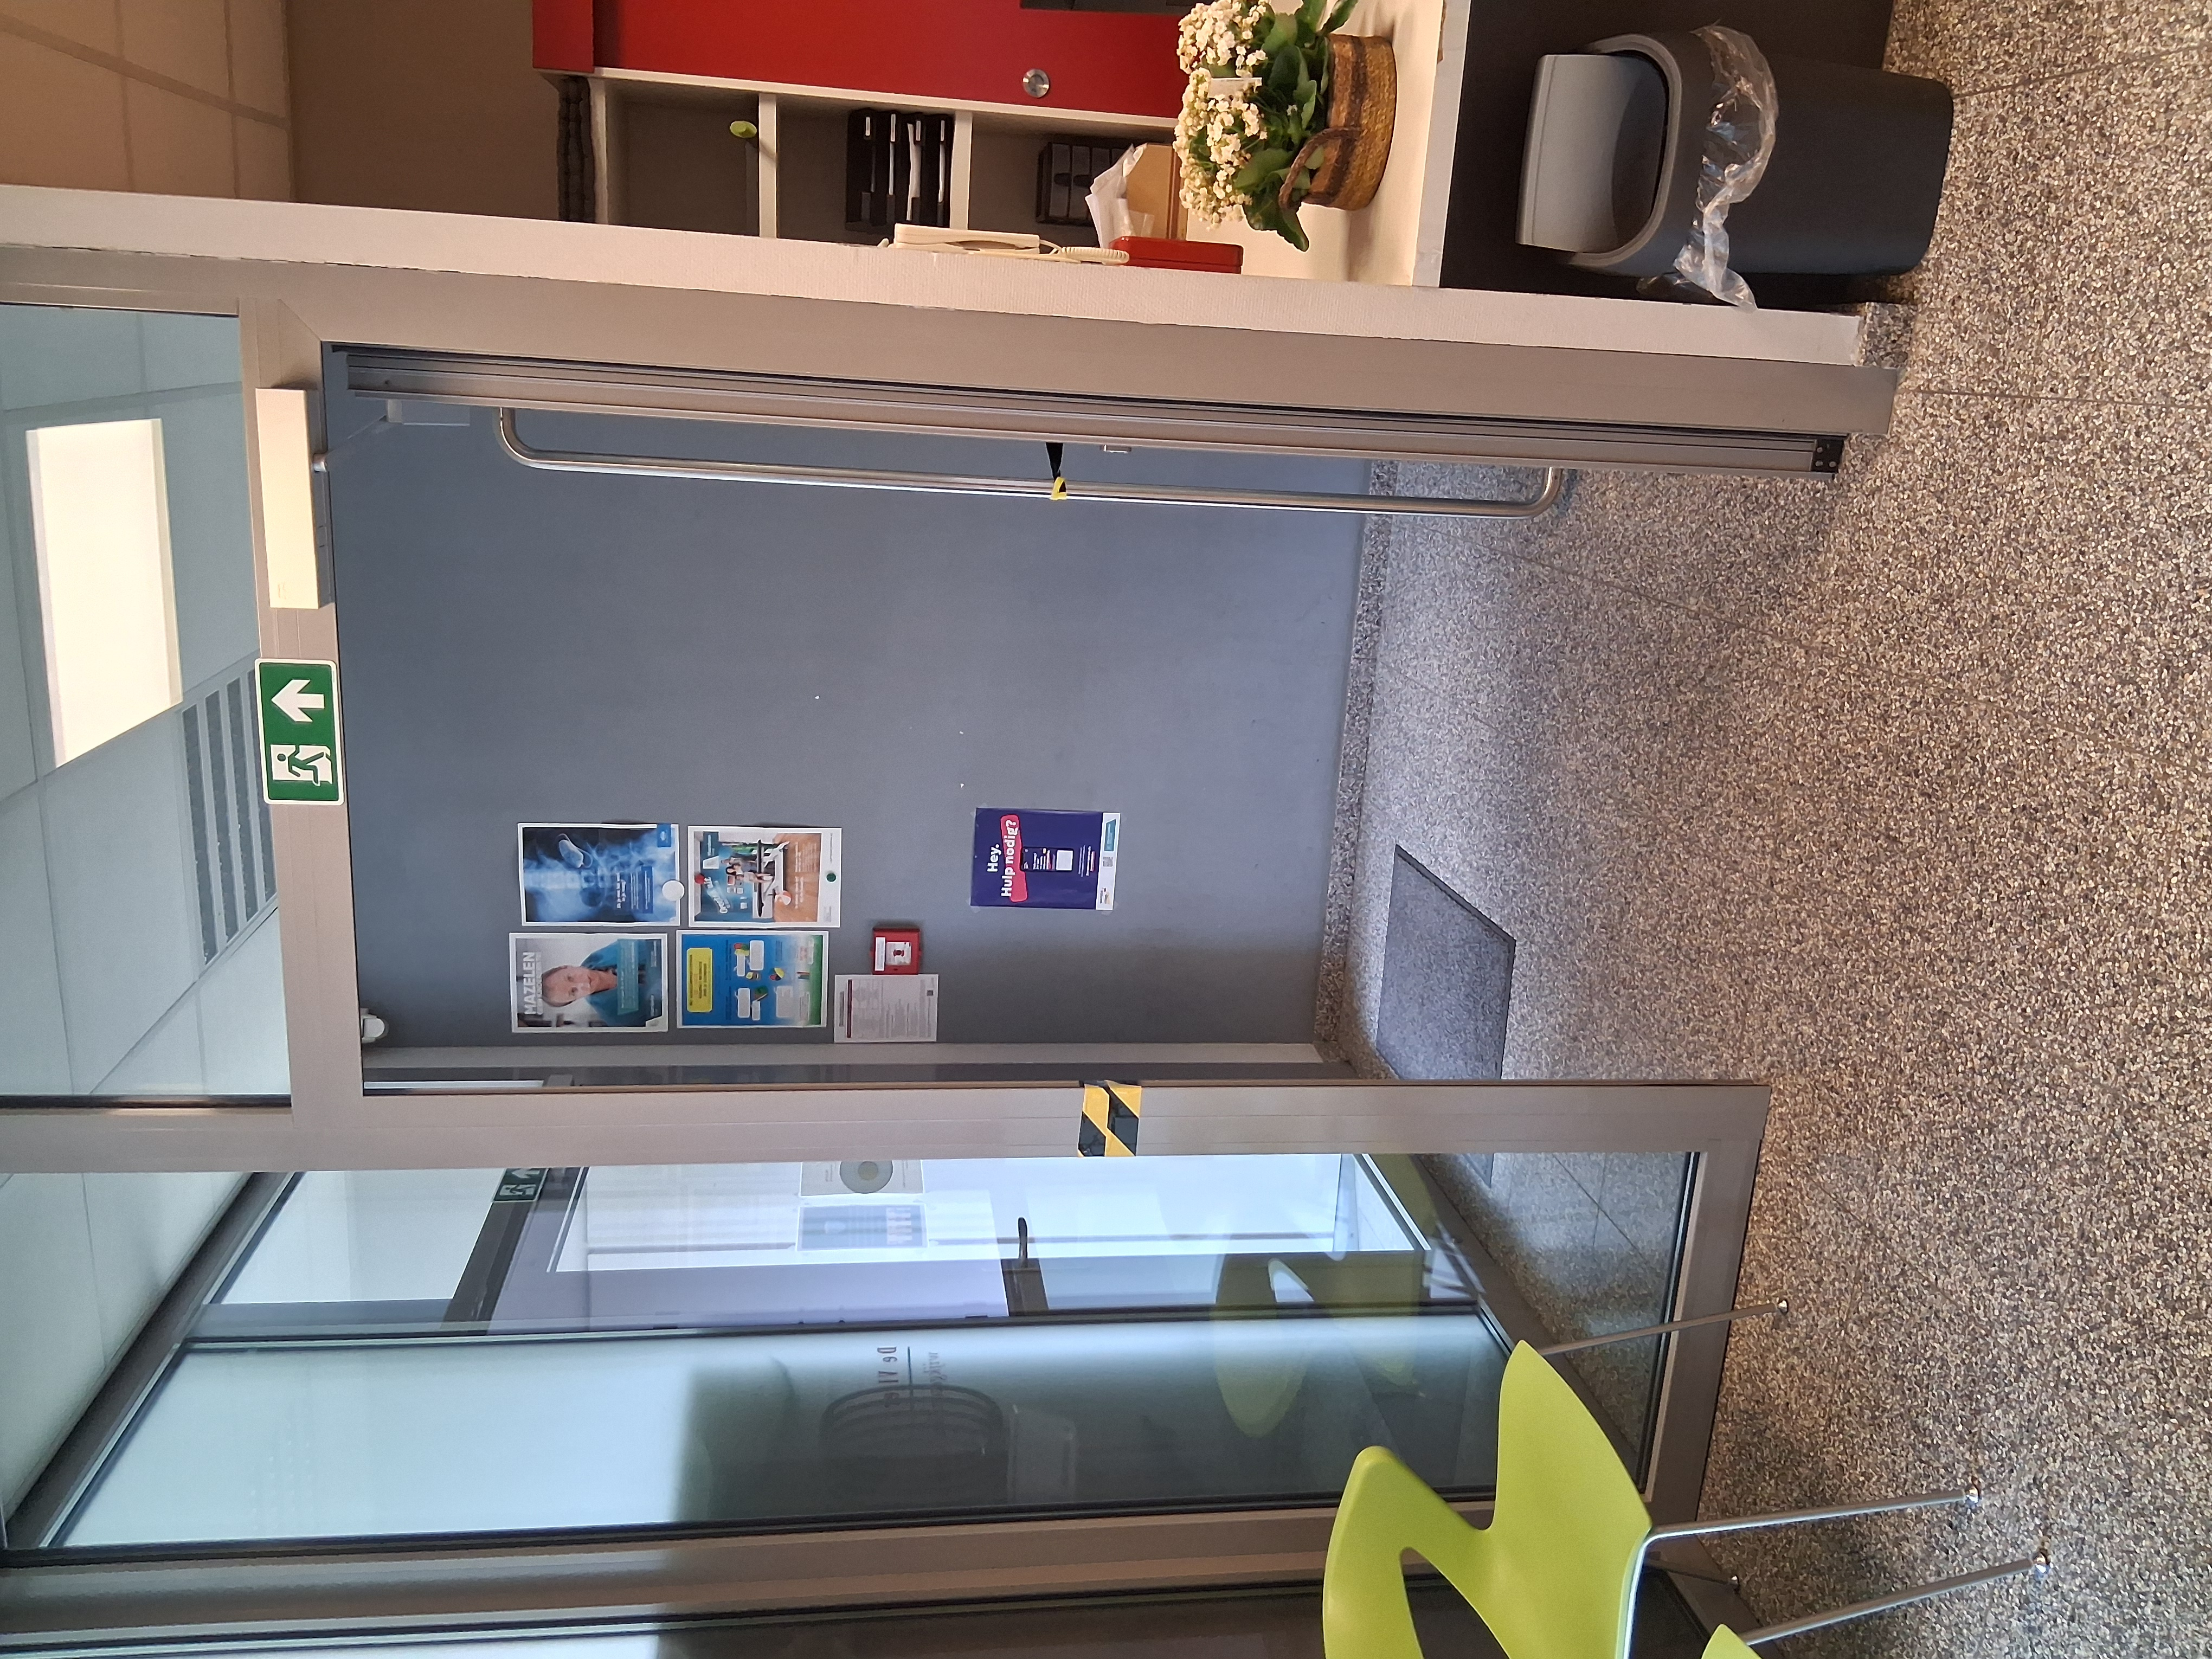
\includegraphics[width=0.4\textwidth]{img/bp/wachtruimtes/ingang.jpg}
    }
    \hspace{0.01\textwidth}
    \rotatebox{270}{%
        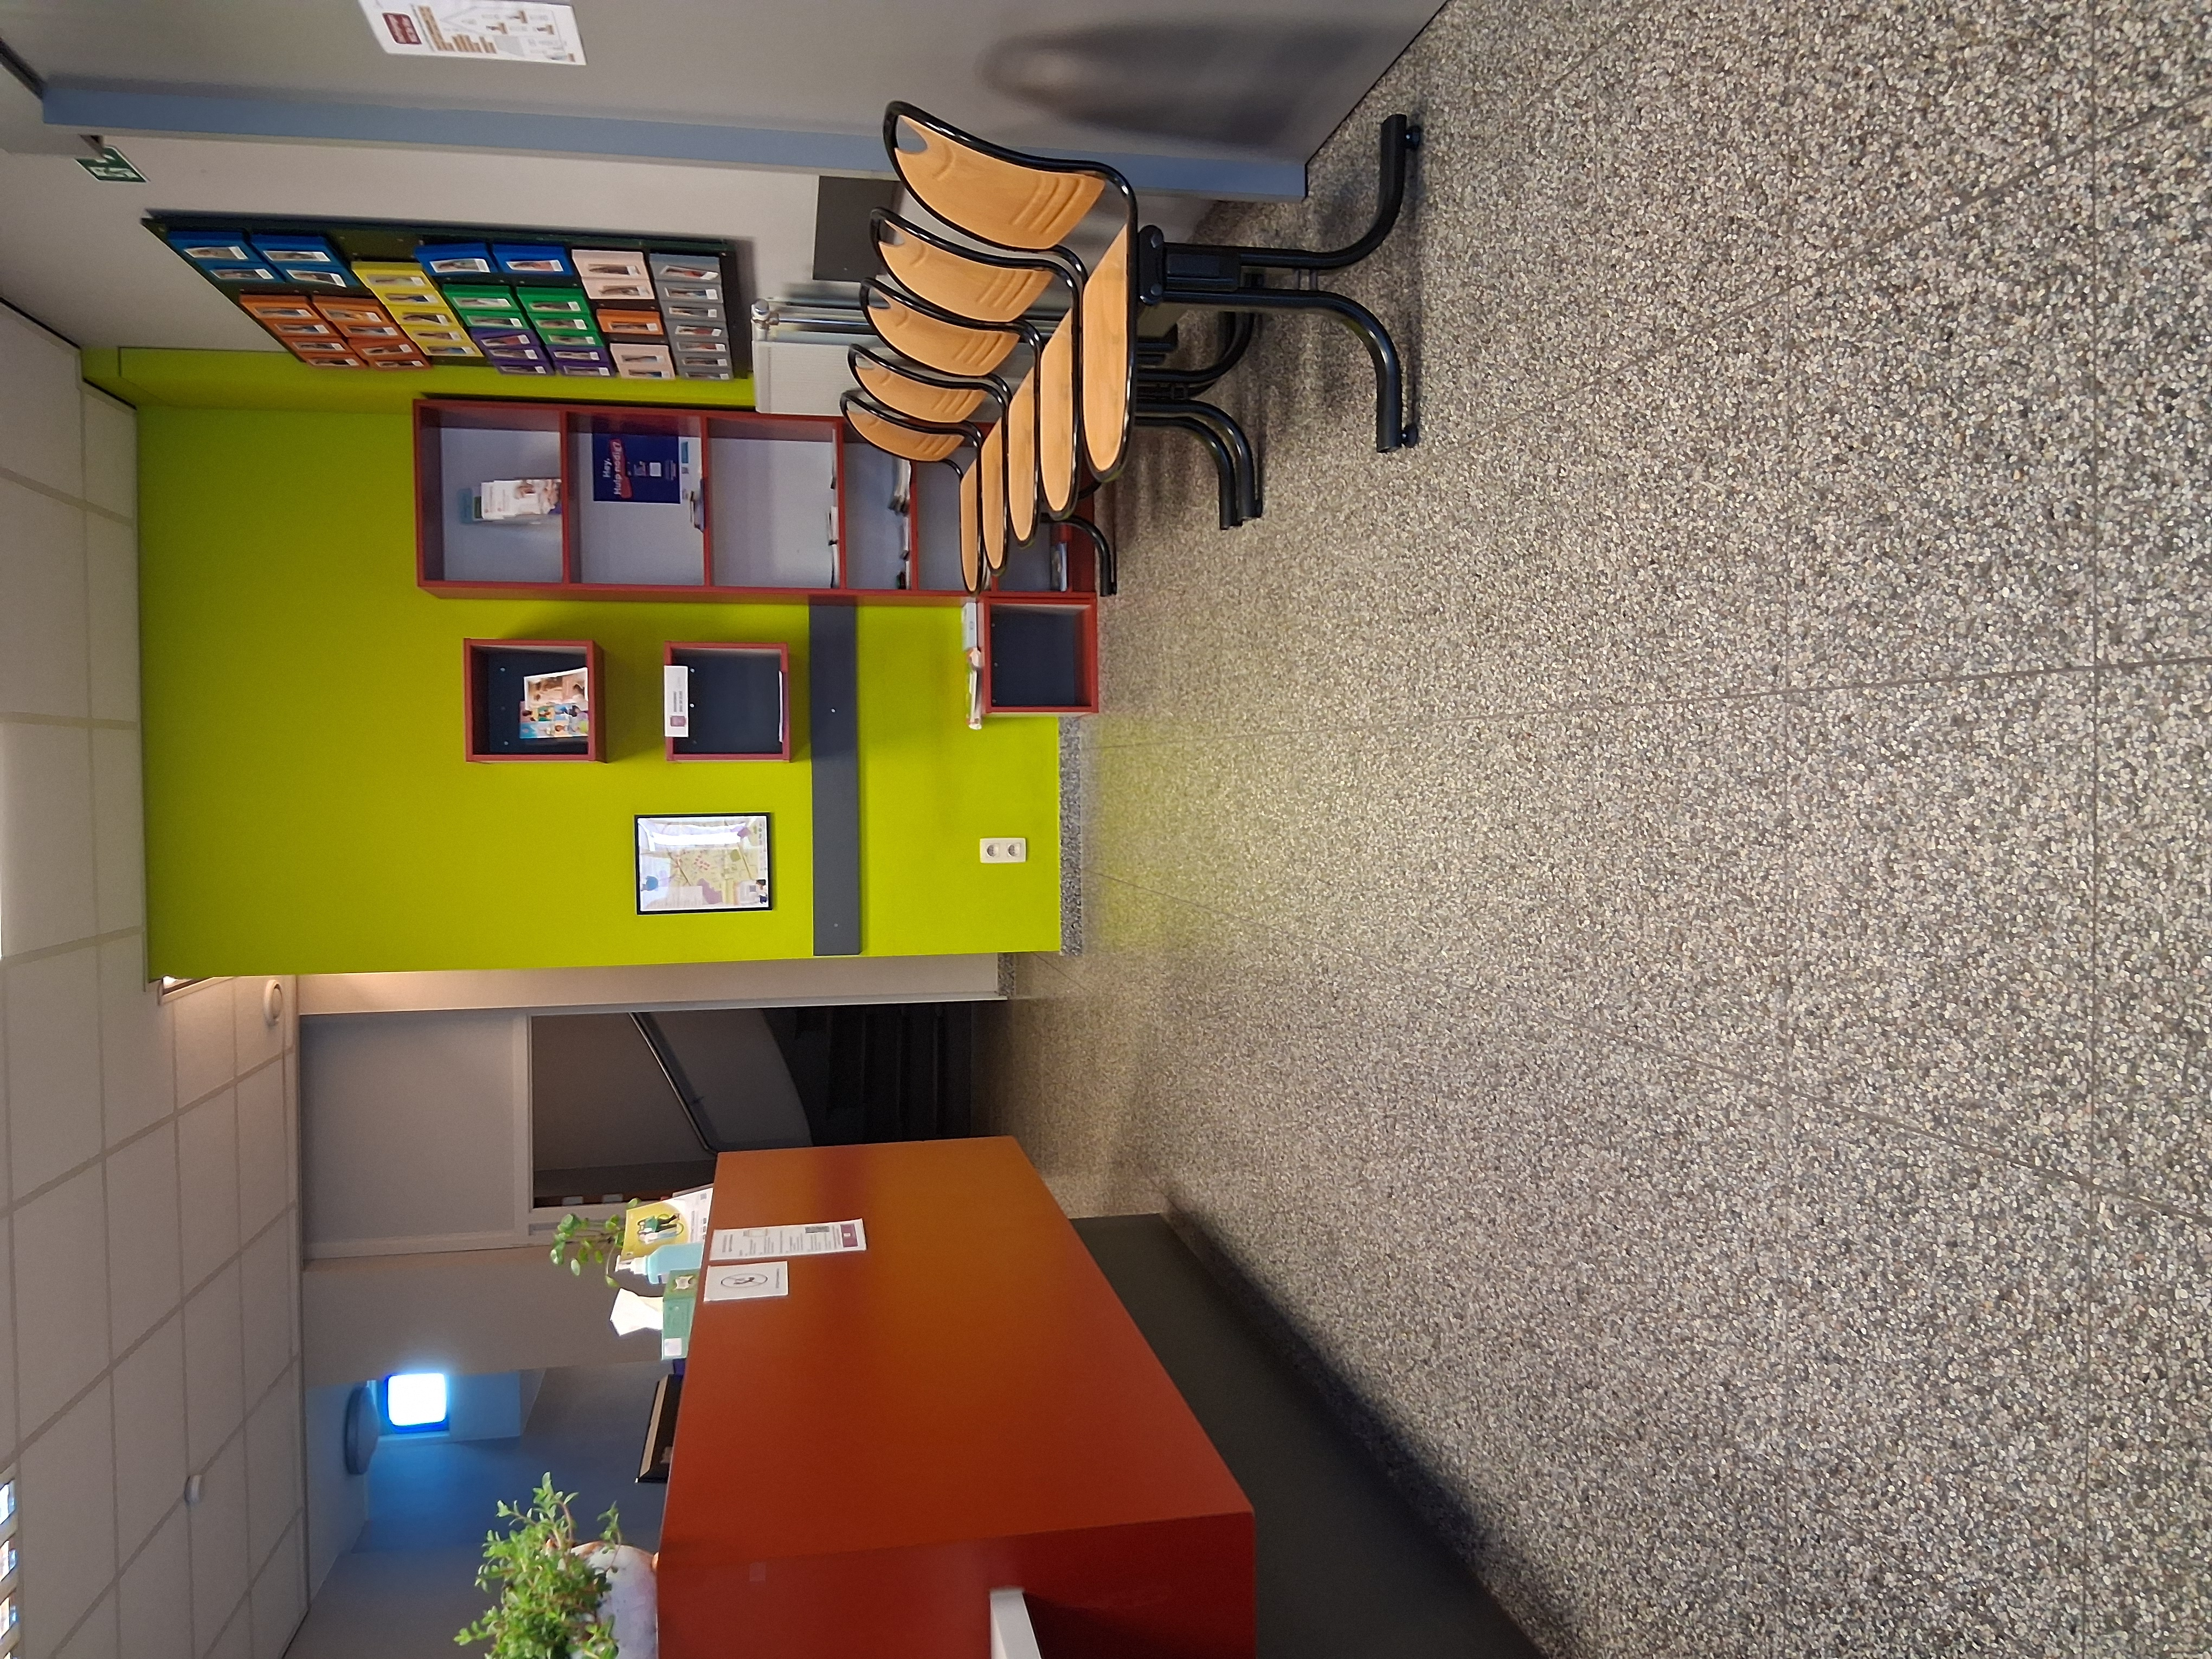
\includegraphics[width=0.4\textwidth]{img/bp/wachtruimtes/wachtruimte.jpg}
    }
    \hspace{0.01\textwidth}
    \rotatebox{270}{%
        \includegraphics[width=0.4\textwidth]{img/bp/wachtruimtes/wachtruimte2.jpg}
    }
    
    \vspace{0.5em} % verticale ruimte tussen bovenste en onderste rij
    
    % Onderste foto
    \rotatebox{0}{%
        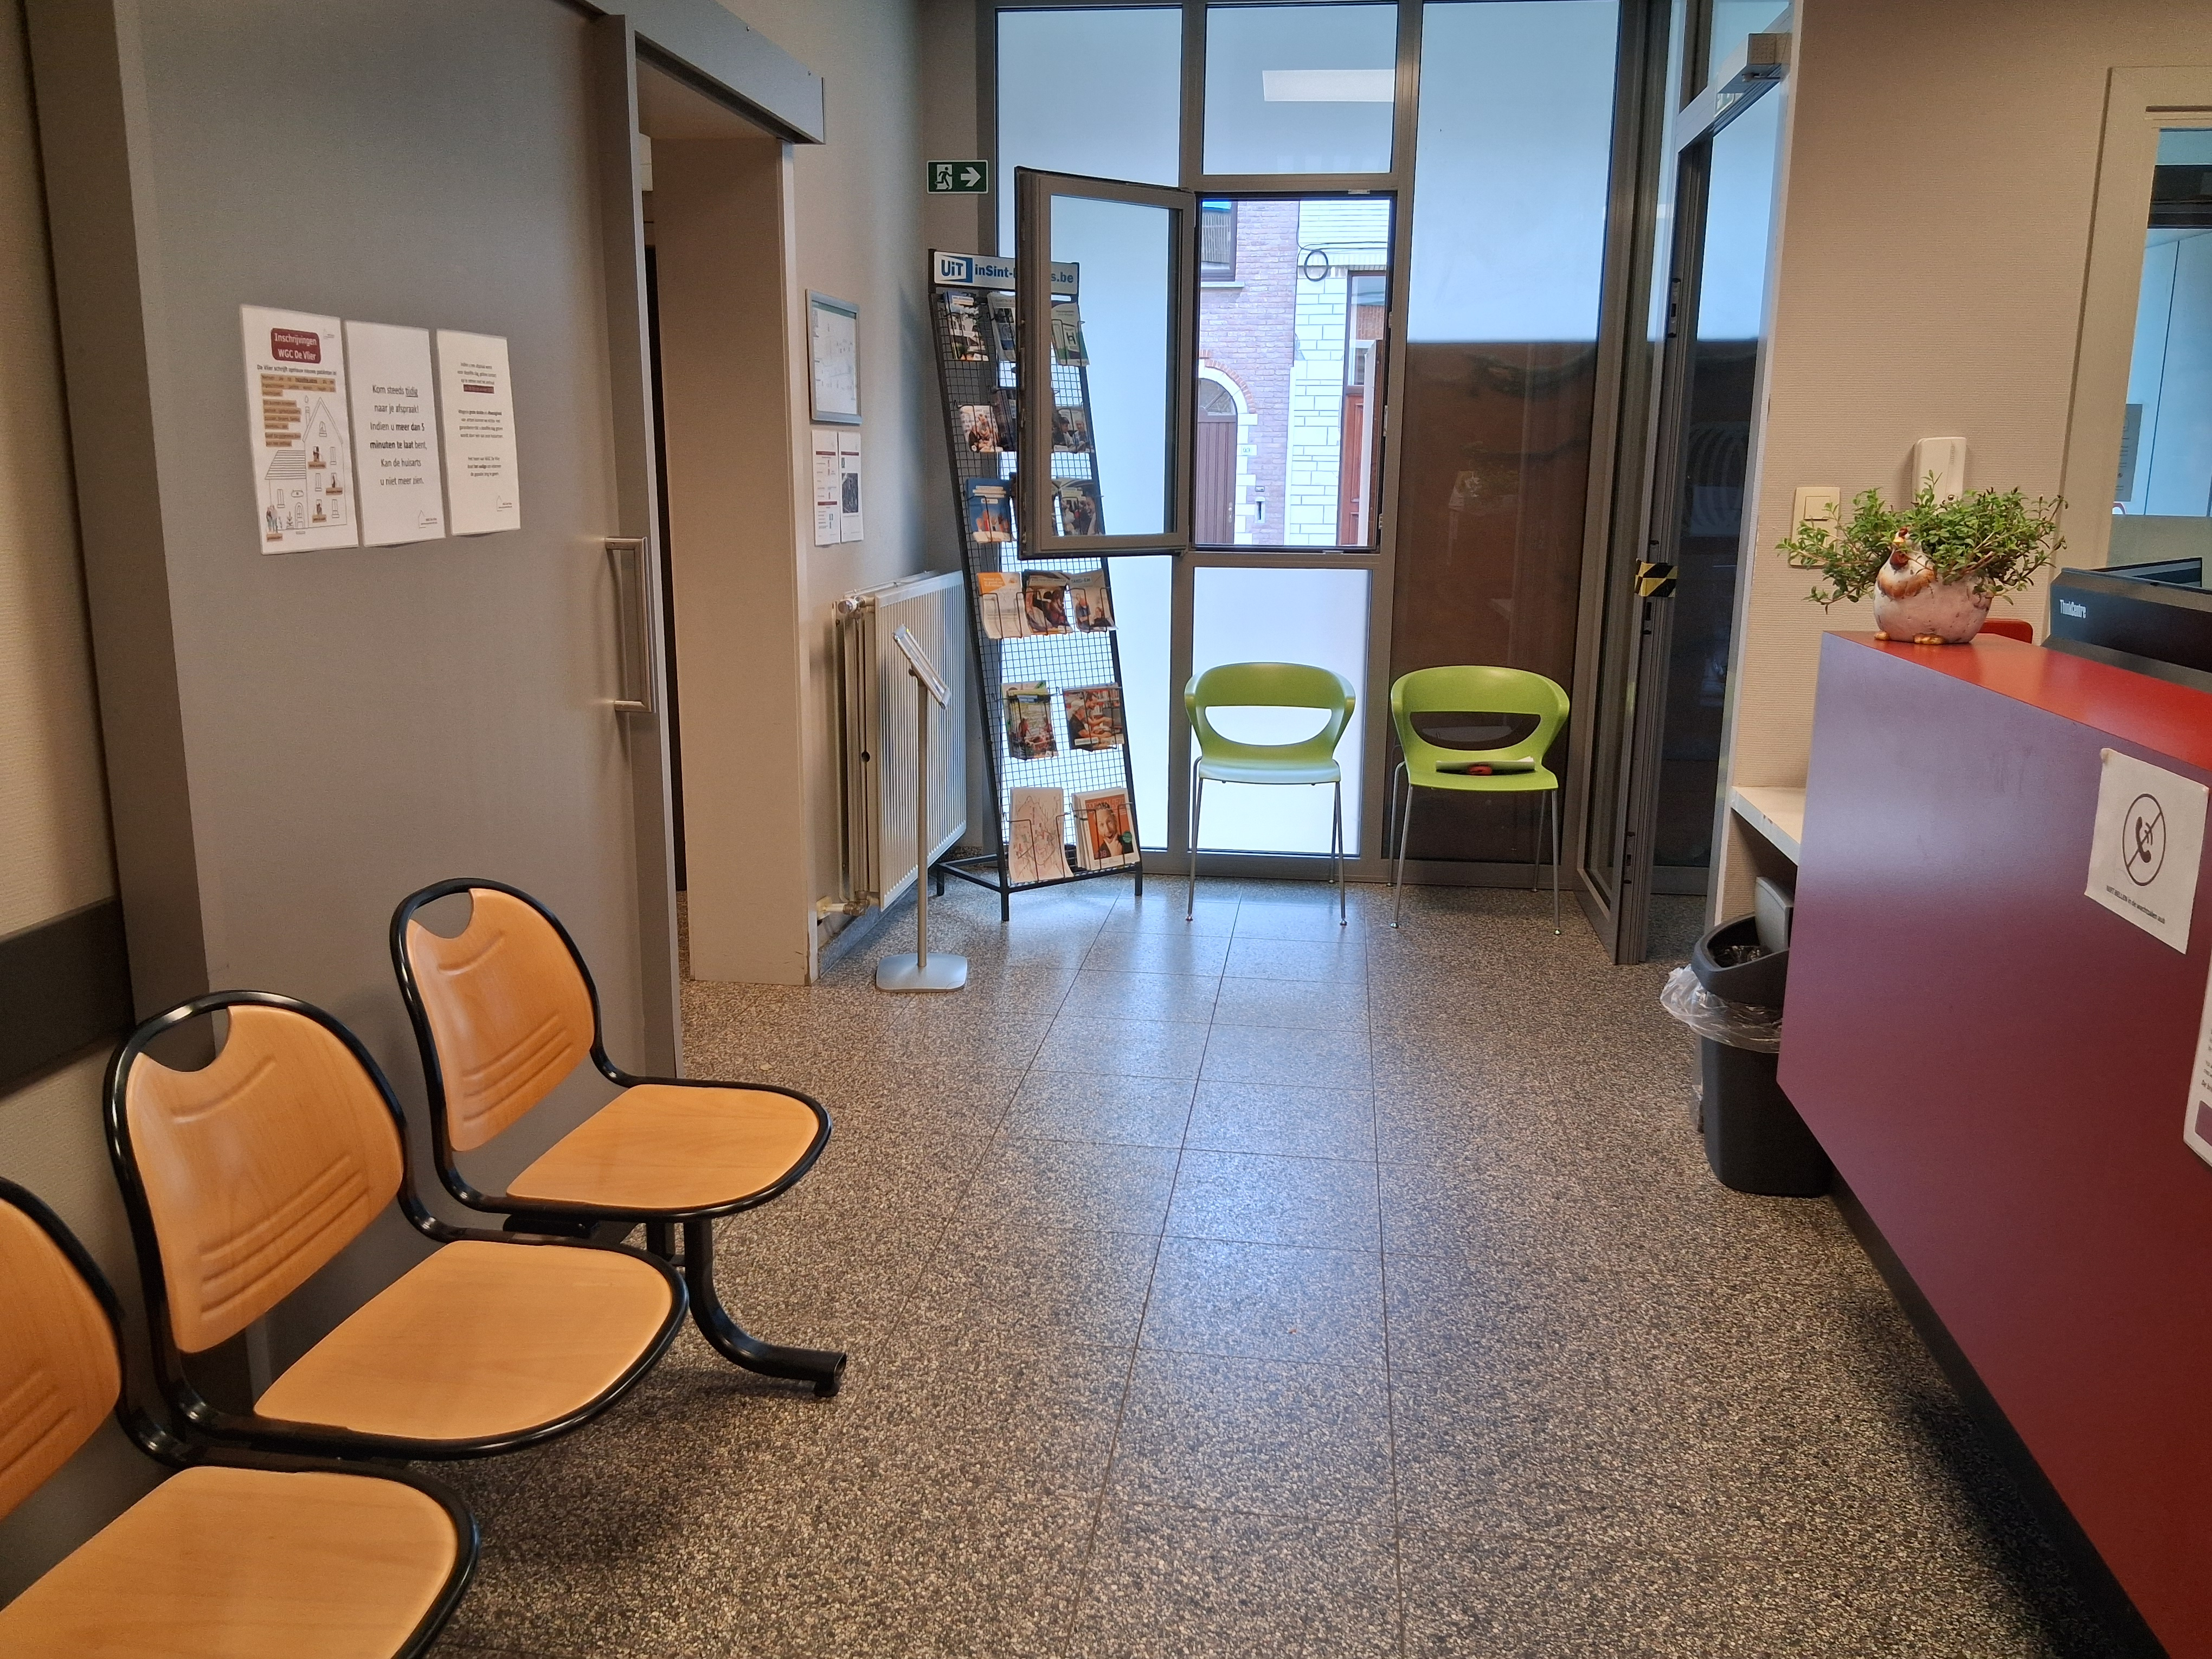
\includegraphics[width=0.46\textwidth]{img/bp/wachtruimtes/wachtruimte1.jpg}
    }
    \rotatebox{0}{%
        \includegraphics[width=0.46\textwidth]{img/bp/wachtruimtes/wachtruimte3.jpg}
    }
    %\caption{Optioneel bijschrift}
    \label{fig:vier_fotos}
\end{figure}
\clearpage

\appendix
\section*{Bijlage B: Fotodocumentatie van de Test-omgeving}
\addcontentsline{toc}{section}{Bijlage B: Fotodocumentatie van de Test-omgeving}

Hieronder volgt een visueel overzicht van de opstelling van het meetsysteem.

\begin{figure}[h!]
    \centering
    % Eerste foto
    \begin{minipage}{0.48\textwidth}
        \centering
        \rotatebox{270}{%
            \includegraphics[width=9cm]{img/bp/wachtruimtes/technische_uitwerking/testomgeving.jpg}
        }
        %\caption{Foto 1} % optioneel
    \end{minipage}
    \hspace{0.02\textwidth}
    % Tweede foto
    \begin{minipage}{0.48\textwidth}
        \centering
        \rotatebox{0}{%
            \includegraphics[width=\linewidth]{img/bp/wachtruimtes/technische_uitwerking/testesp.jpg}
        }
        %\caption{Foto 2} % optioneel
    \end{minipage}
    \begin{minipage}{0.48\textwidth}
        \centering
        \rotatebox{270}{%
            \includegraphics[width=10cm]{img/bp/wachtruimtes/technische_uitwerking/testomgeving1.jpg}
        }
        %\caption{Foto 1} % optioneel
    \end{minipage}
    %\caption{Opstelling van het \gls{iot}-meetsysteem}
    \label{fig:iot_test}
\end{figure}

\clearpage

\appendix
\section*{Bijlage C: Fotodocumentatie van de \gls{iot}-opstelling}
\addcontentsline{toc}{section}{Bijlage C: Fotodocumentatie van de \gls{iot}-opstelling}

Hieronder volgt een visueel overzicht van de opstelling van het meetsysteem.

% Eerste rij van drie foto's (normaal)
\begin{figure}[h!]
    \centering
    \includegraphics[width=0.55\textwidth]{img/bp/wachtruimtes/technische_uitwerking/door.jpg}
    \hspace{0.02\textwidth}
    \includegraphics[width=0.48\textwidth]{img/bp/wachtruimtes/technische_uitwerking/emitters.jpg}
    \hspace{0.02\textwidth}
    \includegraphics[width=0.48\textwidth]{img/bp/wachtruimtes/technische_uitwerking/receivers.jpg}
    \caption{Bovenste rij: deur, emitters en receivers}
\end{figure}

% Tweede rij van drie foto's (geroteerd)
\begin{figure}[h!]
    \centering
    \rotatebox{270}{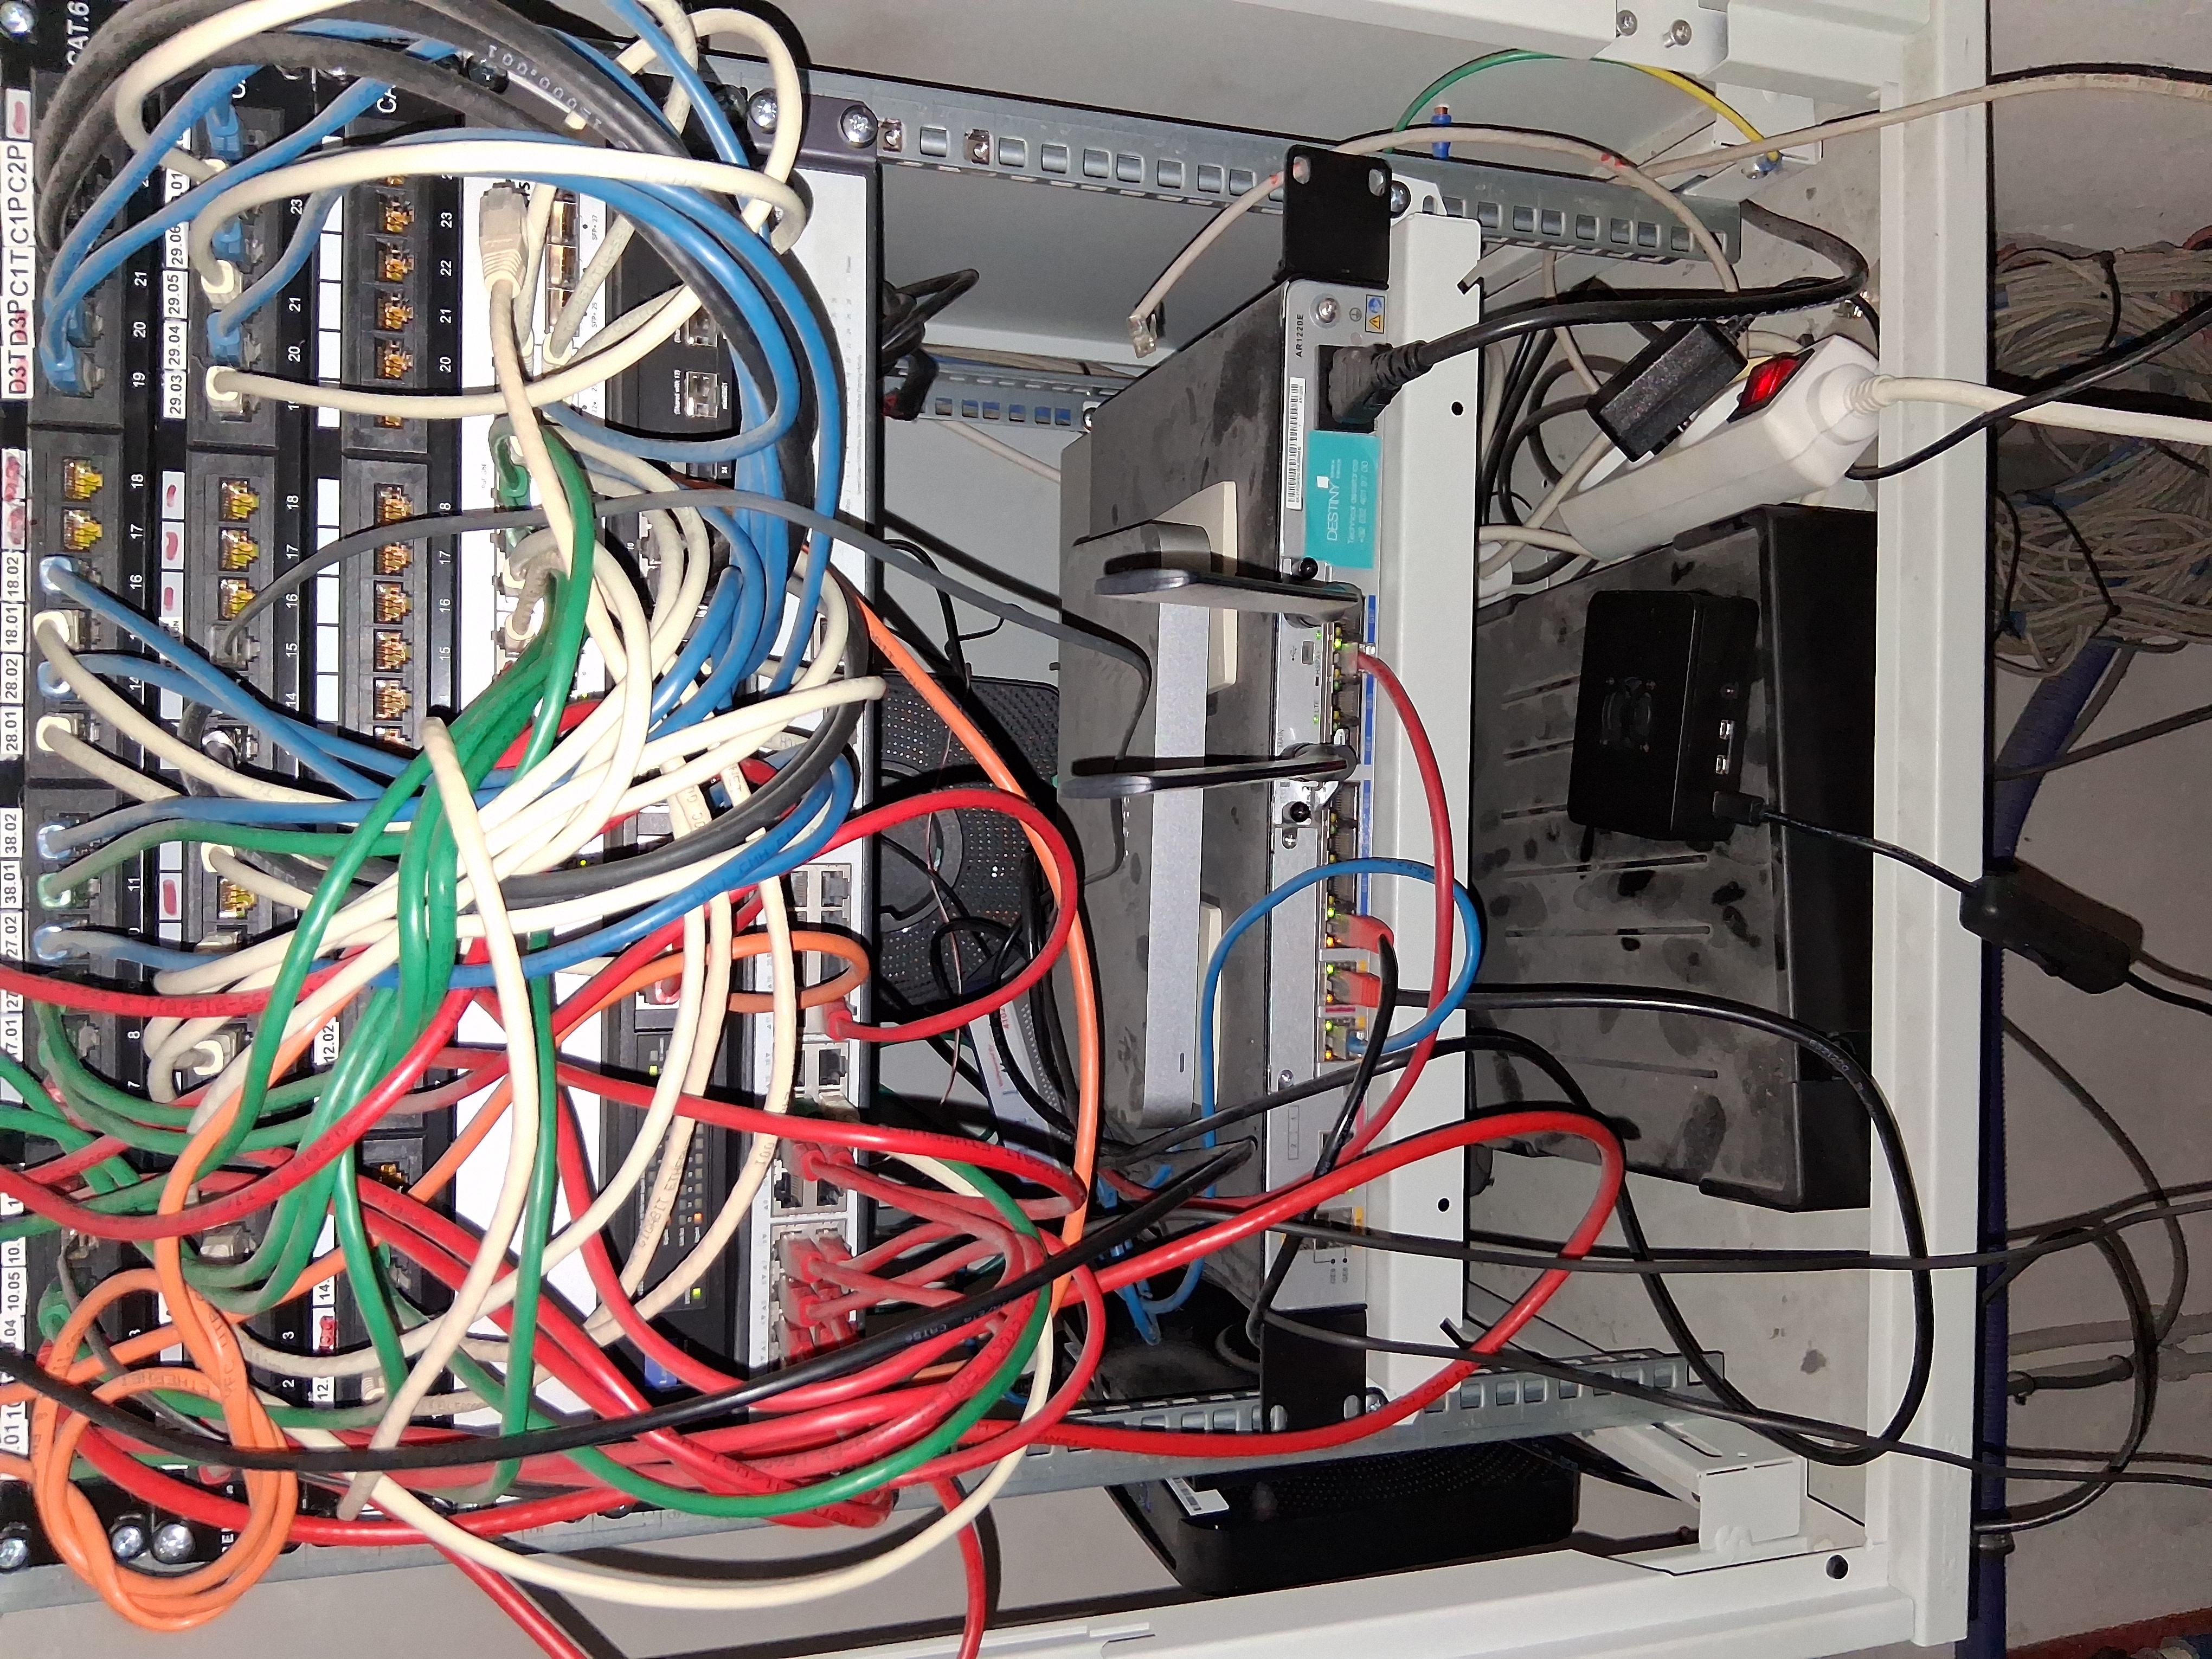
\includegraphics[width=0.6\textwidth]{img/bp/wachtruimtes/technische_uitwerking/pi.jpg}}
    \hspace{0.02\textwidth}
    \rotatebox{270}{\includegraphics[width=0.6\textwidth]{img/bp/wachtruimtes/technische_uitwerking/esp.jpg}}
    \hspace{0.02\textwidth}
    \rotatebox{270}{\includegraphics[width=0.6\textwidth]{img/bp/wachtruimtes/technische_uitwerking/esp1.jpg}}
    \caption{Onderste rij: Raspberry Pi en ESP-modules (geroteerd)}
    \label{fig:foto_iot}
\end{figure}






